\section{The CT18 output: PDFs, QCD parameters, parton luminosities, moments}
\label{sec:OverviewCT18} 

\subsection{Parton distributions as functions of $x$ and $Q$}
\subsubsection{PDFs for individual flavors}
Figure \ref{fig:ct18pdf} shows an overview of the CT18 parton
distribution functions, for $Q = 2$ and $100$ GeV.
The function $x f(x,Q)$ is plotted versus $x$, for flavors $u,
\overline{u}, d, \overline{d}, s = \overline{s}$, and $g$.
We assume $s(x,Q_0)=\bar s(x,Q_0)$, since their difference is
consistent with zero and has large uncertainty \cite{Lai:2007dq}.
The plots show the central fit to the global data listed
in Tables~\ref{tab:EXP_1} and \ref{tab:EXP_2}, corresponding to the
lowest total $\chi^2$ for our choice of PDF parametrizations. These
are displayed with error bands representing the PDF uncertainty at
the 90\% confidence level (C.L.).
%
\begin{figure}[p]
	\center
	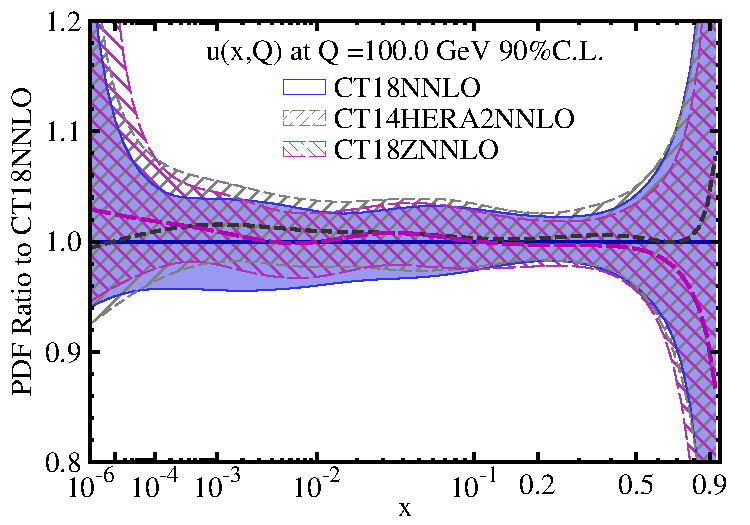
\includegraphics[width=0.49\textwidth]{./fig/u_100_CT18.pdf}
	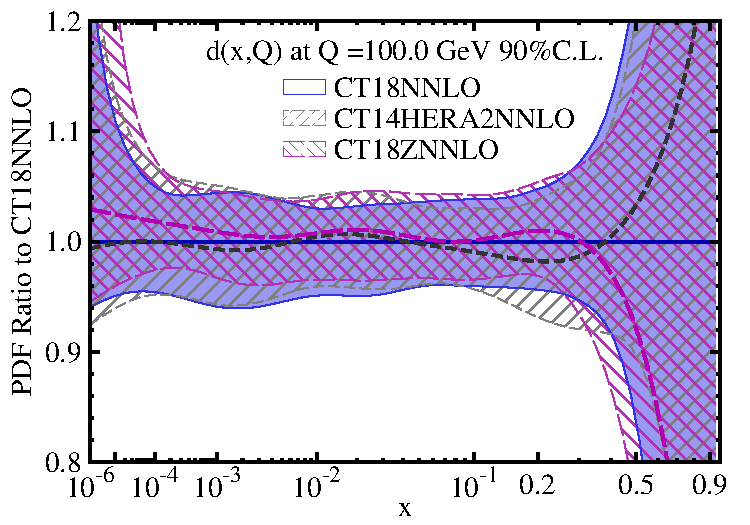
\includegraphics[width=0.49\textwidth]{./fig/d_100_CT18.pdf}
	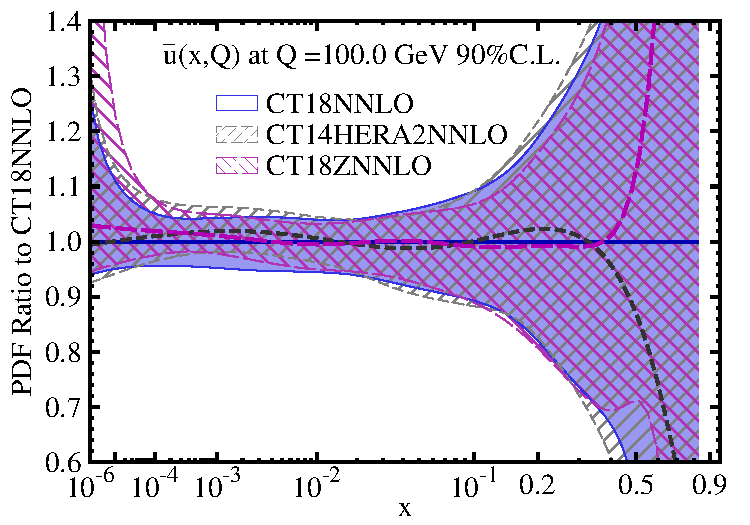
\includegraphics[width=0.49\textwidth]{./fig/ubar_100_CT18.pdf}
	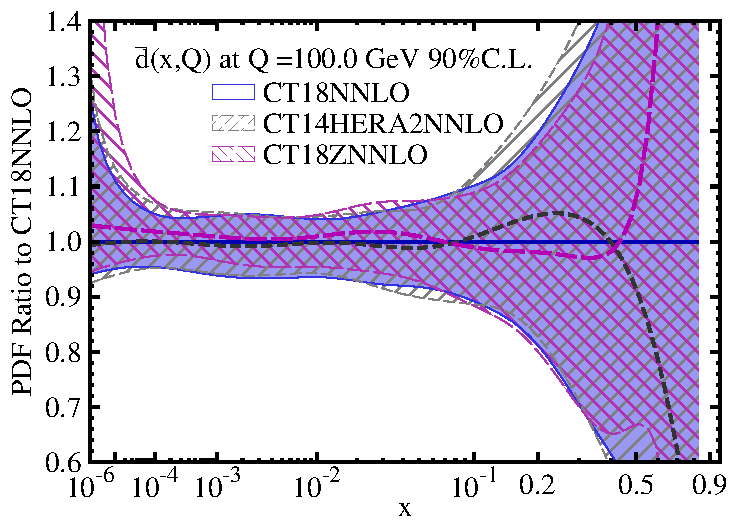
\includegraphics[width=0.49\textwidth]{./fig/dbar_100_CT18.pdf}
	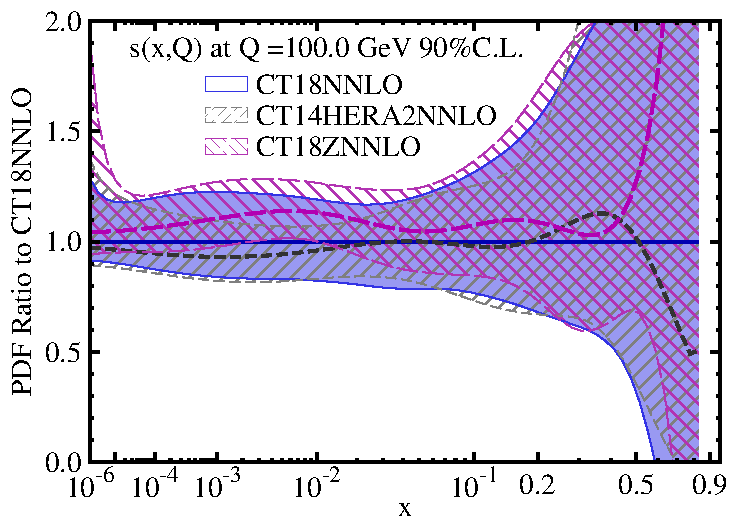
\includegraphics[width=0.49\textwidth]{./fig/s_100_CT18.pdf}
	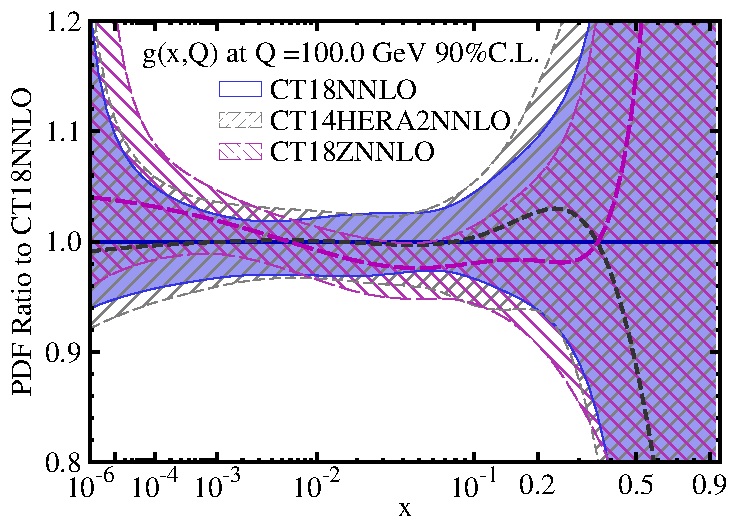
\includegraphics[width=0.49\textwidth]{./fig/g_100_CT18.pdf}
	\caption{A comparison of 90\% C.L. PDF uncertainties from CT18 (violet solid), \CTHERAII (gray short-dashed), and CT18Z (magenta long-dashed) NNLO ensembles at $Q=100$ GeV. The uncertainty bands are normalized to the central CT18 NNLO PDFs.
		\label{fig:PDFbands1}}
\end{figure}


The relative changes from CT14$_\mathrm{HERAII}$ NNLO to CT18 NNLO PDFs are
best visualized by comparing their associated PDF uncertainties. Fig.~\ref{fig:PDFbands1}
compares the PDF error bands at 90\% C.L. for the key flavors, with each band
normalized to the corresponding best-fit CT18 NNLO PDF, represented by the
solid violet line/bands. The long-dashed magenta and short-dashed gray curves/bands correspond
to the CT18Z and CT14$_\mathrm{HERAII}$ NNLO PDFs at $Q=100$ GeV, respectively.


We make a number of observations for the NNLO PDFs. The CT18 $u$ PDF becomes slightly
smaller, compared to \CTHERAII, at almost all $x$ values, with the largest decrease at $x \sim 10^{-3}$.
The $d$ PDF has increased at $x \sim 10^{-3}$ and $x \sim 0.2$, while it slightly decreased at $ x\sim 0.01$. 
The $\bar u$ and $\bar d$ distributions are both smaller at $x \sim 0.3$ and larger at $x \sim 0.05$, 
though the decrease in $\bar d$ is larger. 
Furthermore, except for the $d$ PDF at $ x\sim 0.2$, the error bands of $u$, $d$, $\bar u$ and $\bar d$ 
are about the same as \CTHERAII.
The central strangeness ($s$) PDF has increased for $ x < 0.01$ and decreased for $0.2< x < 0.5$, where  
the strange quark PDF is essentially unconstrained in CT18, just as in \CTHERAII~NNLO.
Also, its uncertainty band is slightly larger than \CTHERAII~for $x > 10^{-4}$, 
as a consequence of the more flexible parametrization and the inclusion of the LHC data.
We have checked that the most important data sets that drive
the abovementioned changes 
in the quark and antiquark PDFs are the LHCb $W$ and $Z$ boson data, as listed in 
Table~\ref{tab:EXP_2} 
with Exp.~IDs=250, 245 and 246, with importance in that order. 
After including the LHCb $W$ and $Z$ boson data, the addition of
CMS 8 TeV $W$ charge-asymmetry data (Exp.~ID=249) leads only to very mild changes in the CT18 PDFs. The central gluon PDF has
decreased in CT18 at $x\approx 0.3$, with a smaller error band at $x \sim 0.1$ and below. 
The decrease of $g$ PDF for $0.1 < x < 0.4$ is caused by the inclusion of CMS and ATLAS jet data (with
Exp.~IDs=545, 543 and 544, in that order) and ATLAS 8 TeV $Z$ boson transverse momentum ($p_T$) data (Exp.~ID=253). 
With the LHC jet data sets already included, adding the ATLAS and CMS top-quark pair data (Exp.~IDs=580 and 573) into the fit does not change the PDFs by a statistically significant amount. 

\subsubsection{Ratios of PDFs}
\begin{figure}[t]
	\center
	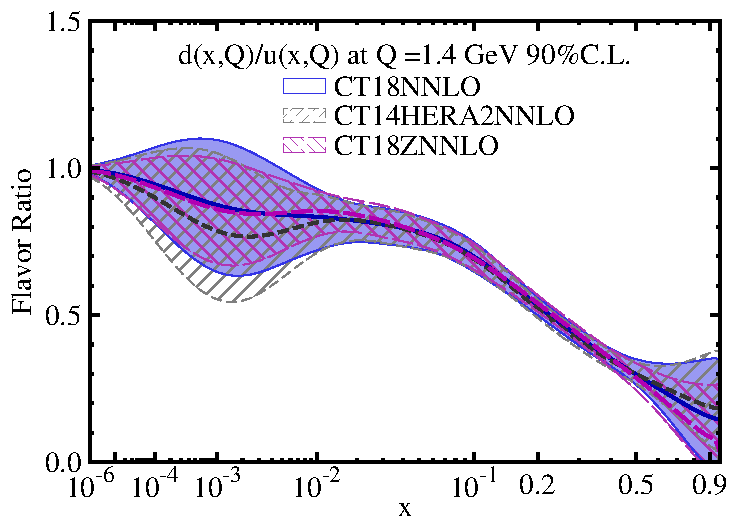
\includegraphics[width=0.49\textwidth]{./fig/du_1p4_CT18.pdf}
	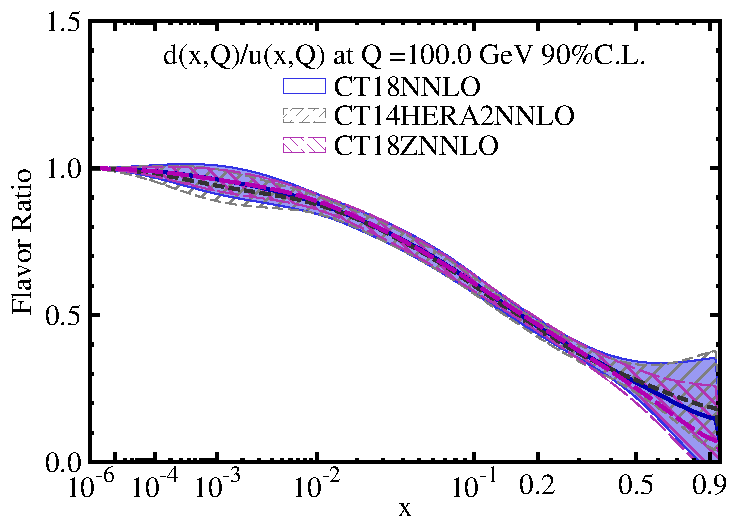
\includegraphics[width=0.49\textwidth]{./fig/du_100_CT18.pdf}
	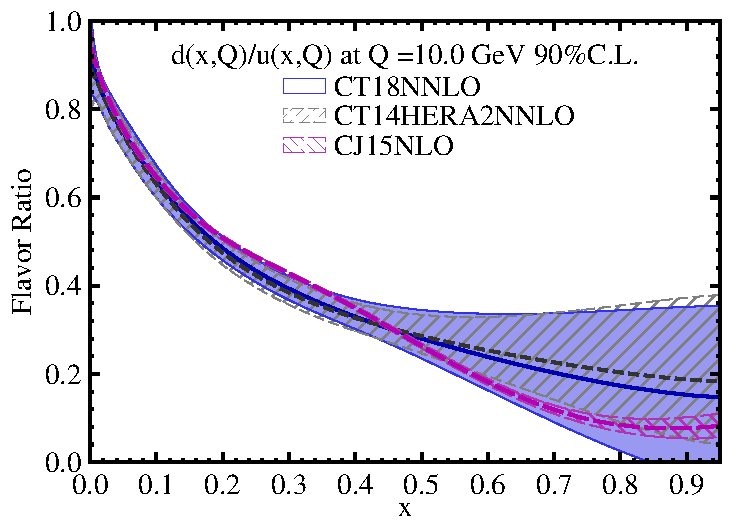
\includegraphics[width=0.49\textwidth]{./fig/pdfs_CT18NNLO_CT14HERA2NNLO_CJ15nlo__10_0GeV_A90CL__10___dou__pdf__lin-lin_ect.pdf}
	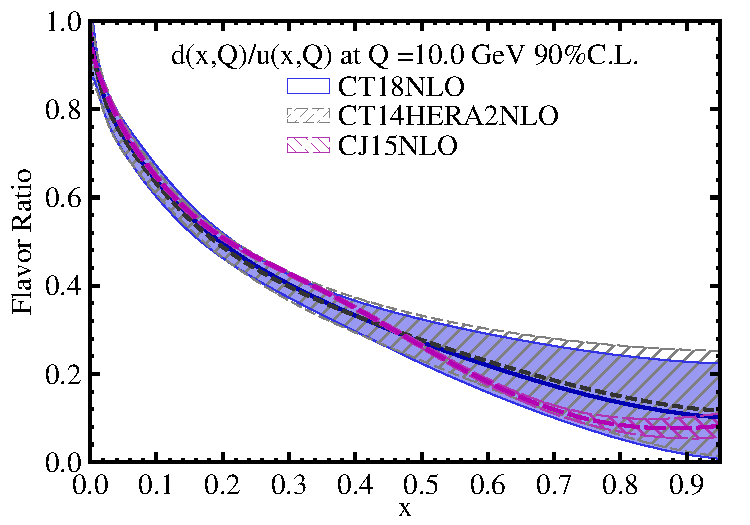
\includegraphics[width=0.49\textwidth]{./fig/pdfs_CT18NLO_CT14HERA2NLO_CJ15nlo__10_0GeV_A90CL__10___dou__pdf__lin-lin_ect.pdf}

	\caption{Top: 90\% C.L. uncertainties on the ratio
		$d(x,Q)/u(x,Q)$ for CT18, \CTHERAII, and CT18Z NNLO ensembles at $Q=1.4$ and $100$ GeV. Bottom: Same, comparing CT18 and \CTHERAII  NNLO ratios (bottom-left) and respective NLO ratios (bottom-right) to the CJ15 NLO ensemble
		at $Q=10$ GeV.
		\label{fig:DOUband}}
\end{figure}

Let us now review the ratios of various
PDFs, starting with the ratio $d/u$ shown in
Fig.~\ref{fig:DOUband}. The changes in $d/u$ from CT18, as compared
to \CTHERAII, can be summarized as a reduction (increase) of the central ratio at $x > 0.5$ ($x<10^{-2}$) and a decreased uncertainty at $x < 10^{-2}$.
Beyond $x=0.5$, the error band of $d/u$ ratio grows,
the parametrization form adopted since CT14 NNLO \cite{Dulat:2015mca}
allows $d/u$ to approach a constant value as $x\rightarrow 1$.
As noted earlier, the parametrization form of $u$, $d$, $\bar u$ and $\bar d$ quarks in CT18 are the same as those in \CTHERAII. 

At such high $x$, the CTEQ-JLab analysis (CJ15) \cite{Accardi:2016qay}
has independently determined the ratio $d/u$ at NLO, by
including the fixed-target DIS data at lower $W$ and higher $x$
that are excluded by the selection cut $W > 3.5 \mbox{ GeV}$ in
CT18,  and by considering higher-twist and nuclear effects
important in that kinematic region. 
Fig.~\ref{fig:DOUband} shows that the central prediction of CT18 
differs from CJ15 at $x > 0.1$. The CT and CJ uncertainty bands are in mutual agreement, even though the error band of CJ15 is much smaller than 
CT18, a fact partly attributable
to the $\Delta \chi^2 = 1$ criterion used in CJ15.
Since the CJ15 PDFs are available only at NLO in $\alpha_s$,
we compare the CJ15 NLO $d/u$ ratios to the respective CT18 NNLO (NLO) ratios in the bottom-left (bottom-right) frame of Fig.~\ref{fig:DOUband}.

\begin{figure}[tb]
	\center
	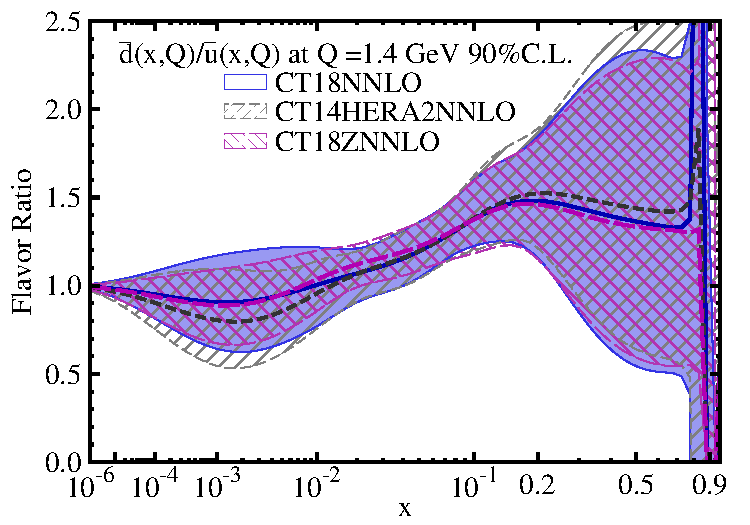
\includegraphics[width=0.49\textwidth]{./fig/dbub_1p4_CT18.pdf}
	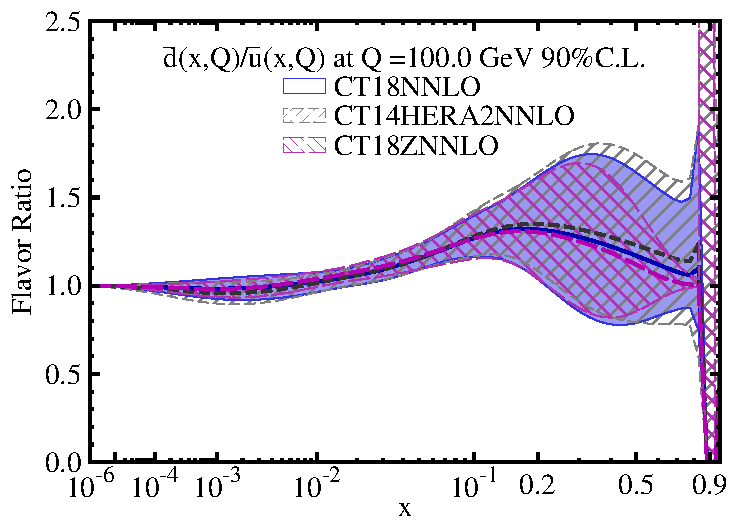
\includegraphics[width=0.49\textwidth]{./fig/dbub_100_CT18.pdf}
	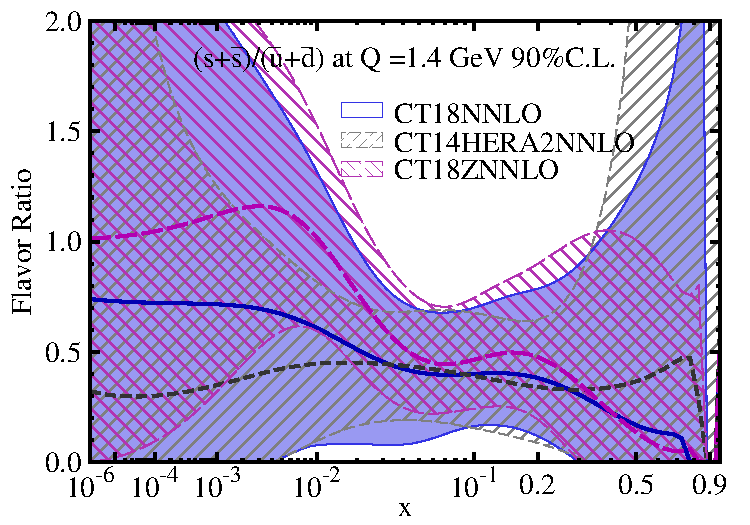
\includegraphics[width=0.49\textwidth]{./fig/Rs_1p4_CT18.pdf}
	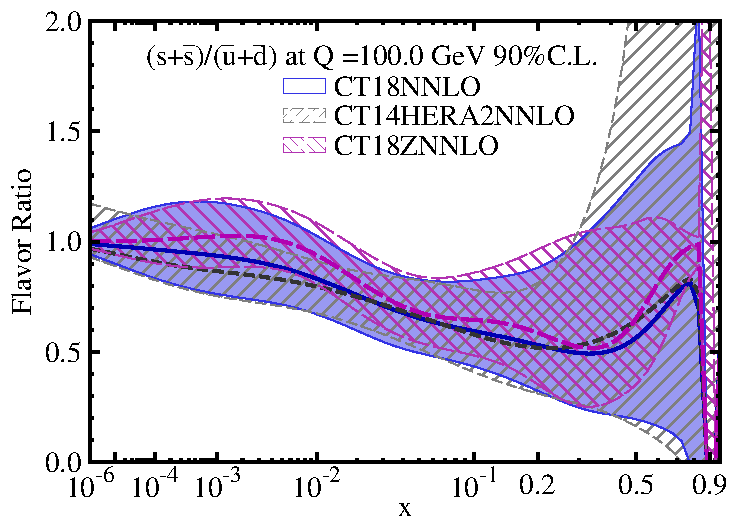
\includegraphics[width=0.49\textwidth]{./fig/Rs_100_CT18.pdf}
	\caption{A comparison of 90\% C.L. uncertainties on the ratios
		$\bar d(x,Q)/\bar u(x,Q)$ and $\left(s(x,Q)+\bar
		s(x,Q)\right)/\left(\bar u(x,Q) +\bar d(x,Q)\right)$,
	for CT18 (solid
		blue), CT18Z (magenta long-dashed), and \CTHERAII~NNLO (gray short-dashed) ensembles
		at $Q=1.4$ or $100$ GeV.
		\label{fig:DBandSBbands}}
\end{figure}


\begin{figure}[tb]
	\center
	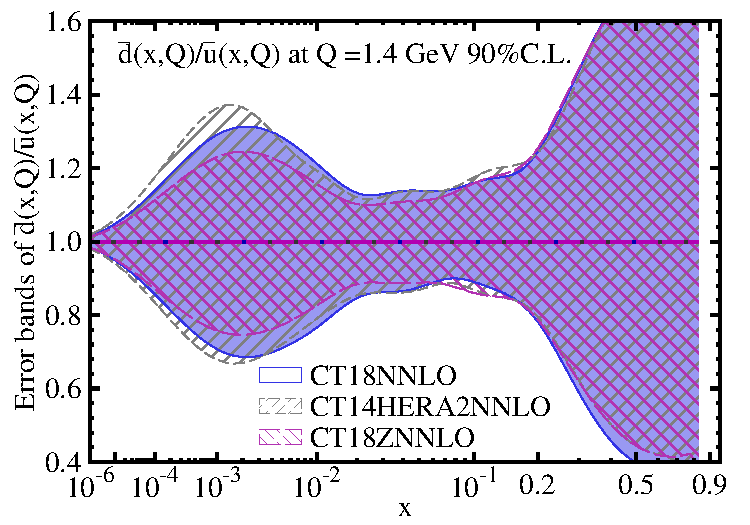
\includegraphics[width=0.49\textwidth]{./fig/dbub_1p4_CT18_err.pdf}
	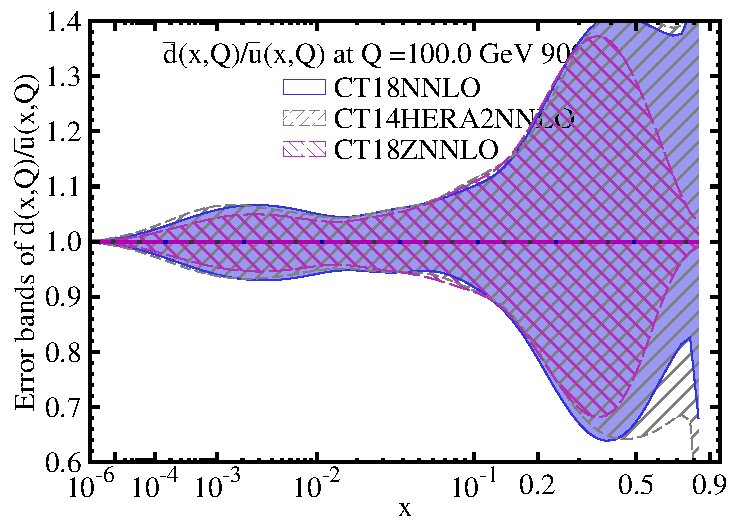
\includegraphics[width=0.49\textwidth]{./fig/dbub_100_CT18_err.pdf}
	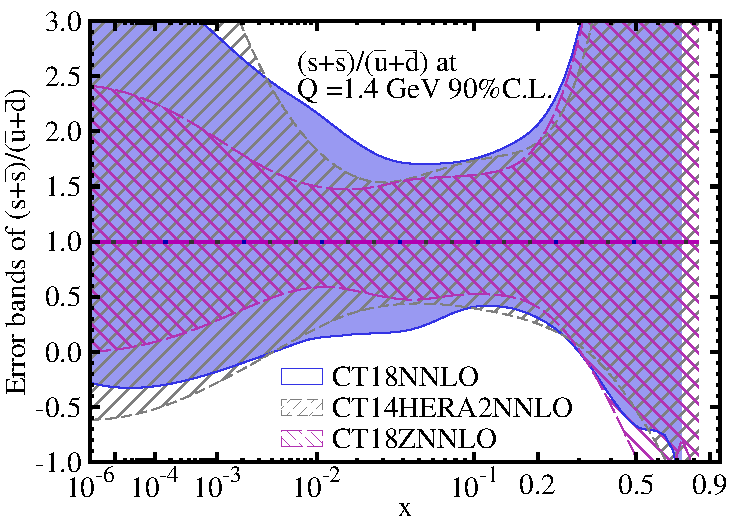
\includegraphics[width=0.49\textwidth]{./fig/Rs_1p4_CT18_err.pdf} 
	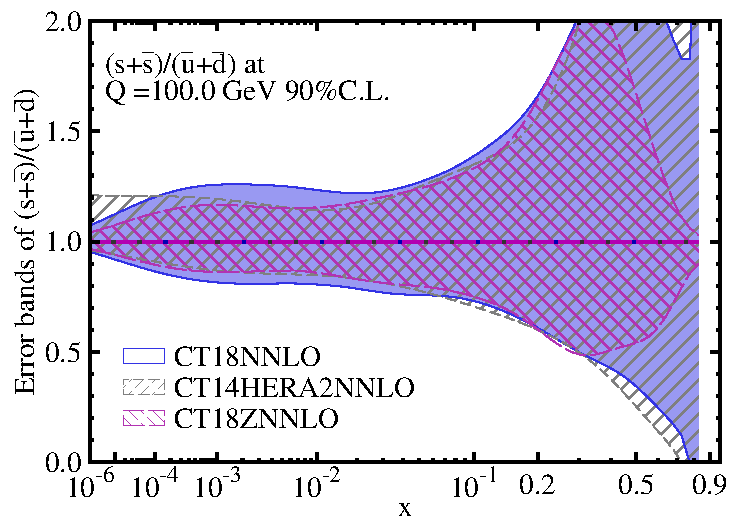
\includegraphics[width=0.49\textwidth]{./fig/Rs_100_CT18_err.pdf} 
	\caption{A comparison of 90\% C.L. uncertainties on the ratios
		$\bar d(x,Q)/\bar u(x,Q)$ and $\left(s(x,Q)+\bar
		s(x,Q)\right)/\left(\bar u(x,Q) +\bar d(x,Q)\right)$,
	for CT18 (solid
		blue), CT18Z (magenta long-dashed), and \CTHERAII~NNLO (gray short-dashed) ensembles
		at $Q=1.4$ or $100$ GeV, relative to 
		their own central fit.  
		\label{fig:DBandSBbands2}}
\end{figure}

%\begin{figure}[tb]
%	\center
%	\includegraphics[width=0.49\textwidth]{./fig/ub_1p4_CT18.pdf}
%	\includegraphics[width=0.49\textwidth]{./fig/ub_1p4_CT18_err.pdf}
%	\includegraphics[width=0.49\textwidth]{./f%ig/db_1p4_CT18.pdf}
%	\includegraphics[width=0.49\textwidth]{./fig/db_1p4_CT18_err.pdf}
%	\includegraphics[width=0.49\textwidth]{./fig/s_1p4_CT18.pdf}
%	\includegraphics[width=0.49\textwidth]{./fig/s_1p4_CT18_err.pdf}
%	\caption{A comparison of 90\% C.L. uncertainties on $\bar u(x,Q)$, $\bar d(x,Q)$ and $s(x,Q)$
%	for CT18 NNLO (solid
%		blue), CT18Z NNLO (magenta long-dashed), and \CTHERAII~NNLO (gray short-dashed) ensembles
%		at $Q=1.4$ GeV,
%		relative to the CT18 NNLO central fit in the left panels and to their own central fits in the right. 
%		\label{fig:UDSBand}}
%\end{figure}

Turning now to the ratios of sea quark PDFs in
Fig.~\ref{fig:DBandSBbands}, we observe that the uncertainty on $\bar
d(x,Q)/\bar u(x,Q)$ in the left inset has decreased at small $x$
in CT18. For $x\! >\! 0.1$, the CT18 nonperturbative parametrization forms for $\bar u$ and $\bar d$ ensure that the ratio
$\bar d(x,Q_0)/\bar u(x,Q_0)$ can approach a constant value, which
turns out to be close to 1 in the central fit. The uncertainty on
$\bar d/\bar u$ has also decreased, most notably for $x\! \gtrsim\! 10^{-3}$, primarily due to the inclusion
of the LHCb data sets (Exp.~IDs=250, 245 and 246), cf.~the upper-left panel of Fig.~\ref{fig:DBandSBbands2} at $Q\!=\!1.4\,\mathrm{GeV}$.


The overall increase in the strangeness PDF at $ x < 0.03$ and decrease of $\bar u$ and $\bar d$ PDFs at $ x  < 10 ^{-3}$, cf.~Fig.~\ref{fig:PDFbands1}, lead to a
larger ratio of the strange-to-nonstrange sea quark PDFs,
\begin{equation}
	R_s(x,Q) \equiv \frac{s(x,Q) + \bar{s}(x,Q)}{\bar{u}(x,Q) + \bar{d}(x,Q)}\ ,
\label{eq:Rs}
\end{equation}
presented in
Fig.~\ref{fig:DBandSBbands}. 
$R_s(x,Q)$ measures the $x$ and $\Q$ dependence of the breaking of flavor-$\mathrm{SU}(3)$ symmetry,
with older analyses typically fixing $R_s = 0.5$. More recently, a number of previous CTEQ
studies \cite{Lai:2007dq,Olness:2003wz} examined contemporary constraints on $R_s$,
particularly driven by the neutrino-induced SIDIS dimuon production measurements by the CCFR and NuTeV Collaborations, but also by precise inclusive HERA measurements. 
These works found significant evidence of an independent $x$ dependence for $s^+(x)\! \equiv\! s(x)\! +\! \bar{s}(x)$, distinct from $\bar{u}\!+\!\bar{d}$, 
but were unable to exclude a vanishing strangeness momentum fraction  asymmetry,
$\langle x \rangle_{s^-}\! =\! \int^1_0 dx\ x [s-\bar{s}](x,\Q=m_c)\! =\! 0$.
%
%

In the present work, we continue to assume $s^-(x,Q)=0$ and focus on $s^+(x,Q)$
and the related $R_s(x,Q)$, the quantities that
both reflect the interplay of the older charged-current DIS data and new LHC measurements that are detailed later in Sec.~\ref{sec:Quality} and App.~\ref{sec:AppendixCT18Z}.
Here let us mention that, at $ x  \ll 10 ^{-3}$, the $R_s$
ratio is determined entirely by the parametrization form and was found
in CT10 to be consistent with the exact $\mathrm{SU}(3)$ symmetry of PDF
flavors, $R_s(x,Q) \rightarrow 1$
at $x\rightarrow 0$, albeit with a large uncertainty. 
The $\mathrm{SU}(3)$-symmetric asymptotic solution at $x\rightarrow 0$
was not enforced in CT14 or \CTHERAII, so that their $R_s$ ratio  
was around $0.3$ to $0.5$ at $x\approx 10^{-5}$ and $Q=1.4$ GeV.
In CT18, we have assumed a different $s$-PDF nonperturbative
parametrization form (with one more parameter added), but the one that
still ensures a stable behavior of $R_s$ for $x\! \to\! 0$, so that
$R_s (x \to 0)$ is about 0.7 and 1, respectively, in CT18 and CT18Z
fits. 

\subsubsection{Changes in the $x$ dependence of PDFs, summary}
We may summarize the pulls of specific processes on the central CT18 fit as follows. 

\begin{itemize}

\item The most noticeable overall impact of the LHC inclusive jet
  production on the central gluon PDF $g(x,Q)$ is to mildly reduce it
  at $x > 0.2$ within the original PDF uncertainty band. The pulls
  from the jet data sets change little after the decorrelation of some
  systematic errors, cf. Sec.~\ref{sec:DataJets},
  and when the $0.5\%$ MC uncertainty on theory values is added.
The pulls from various jet data sets on $g(x,Q)$ neither follow a
uniform trend across the whole $x$ range nor are consistent among
various measurements, as is demonstrated, e.g., by the $L_2$
sensitivity in Fig.~\ref{fig:L2glu} and LM scans in
Sec.~\ref{sec:QualityOverview}. 

\item The LHCb data, combined over all processes, have some impact on
  the $u$, $d$ and $s$ quarks, and pull the $s (x,Q)$ up at small $x$.   

\item The ATLAS 8 TeV $Z$ $p_T$ data (Exp.~ID=253), for the nominal
  QCD scales assumed in the CT18 NNLO fits, weakly pull the gluon PDF
  at $x>0.05$ downward, in the direction similar to the average pull
  of the LHC inclusive jet data. The relative magnitude of the pull
  from these data, as compared to those from the jet experiments,
  can be estimated from the $L_2$ sensitivity plot
  for $g(x,Q)$ in Fig.~\ref{fig:L2glu}.

\item The ATLAS 7 TeV data on $W$ and $Z$ rapidity distributions
  (Exp.~ID=248), included only in CT18A and Z, have the largest
  influence on the PDFs, as discussed in
  App.~\ref{sec:AppendixCT18Z}. The directions of their pulls are
  similar to LHCb. 

\item The LHC data on $t \bar t$ double differential cross sections
  also appears to favor a softer gluon at large $x$, but the pull is
  not statistically significant, {\it i.e.}, much weaker than that of
  the inclusive jet data with its much larger number of data points.  

\end{itemize}

These constraints are further explored in depth in
Sec.~\ref{sec:QualityOverview} using a combination of statistical techniques.

\subsection{The global fits for $\alpha_s$ and $m_c$}
\label{sec:AlphasDependence}

\begin{figure}[tbp]
\centering
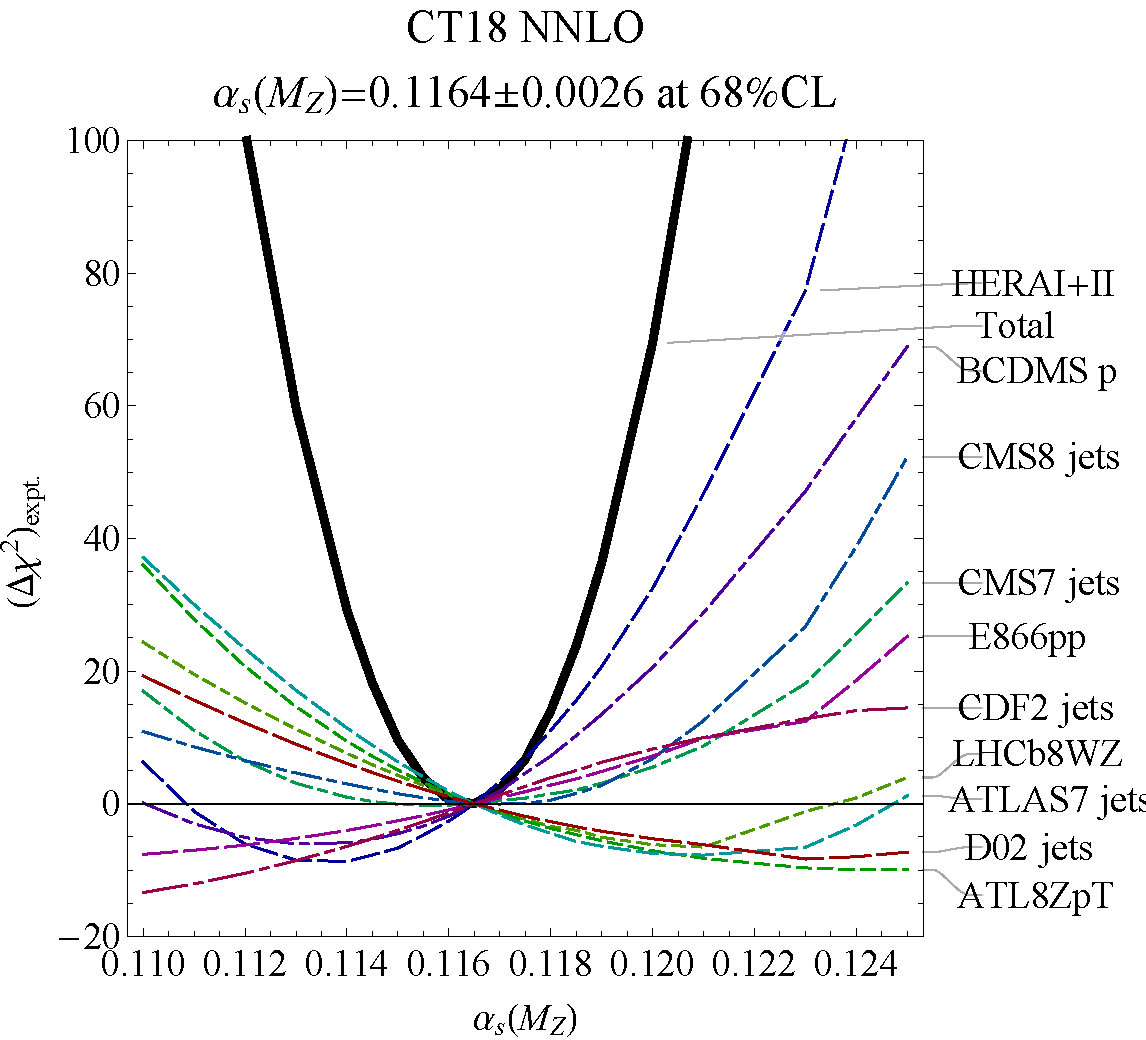
\includegraphics[width=0.49\textwidth]{./fig/alphas_scanTct18_pjb05a.pdf} \ \
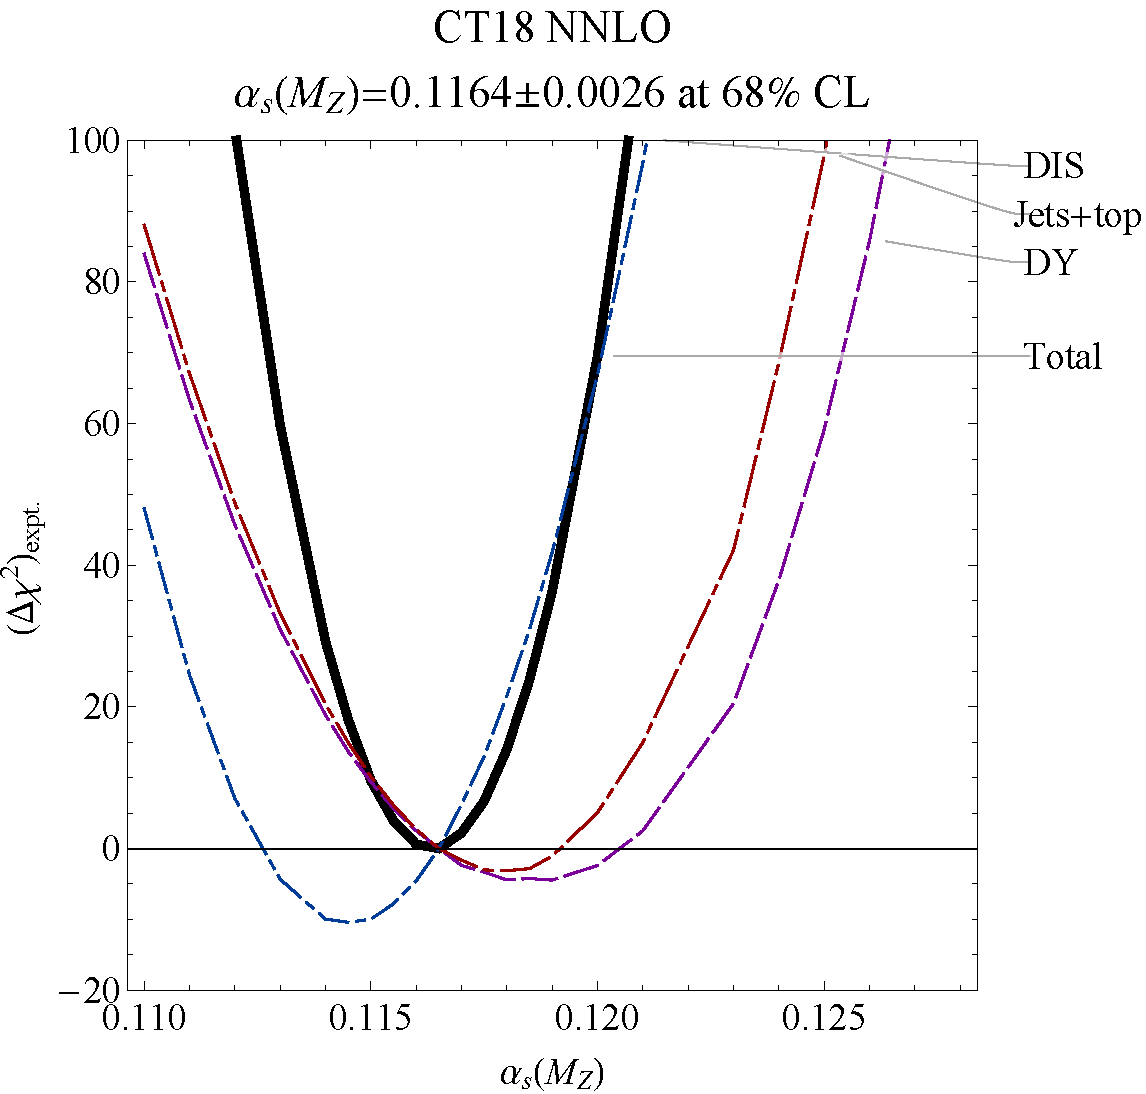
\includegraphics[width=0.46\textwidth]{./fig/alphas_scanTct18_pjb05a2.pdf}
\caption{The scan of the strong coupling constant at the scale of $M_Z$ for CT18 at NNLO. Left: changes of $\chi^2$ of all the data sets together
    (heavy black line) and of several individual experiments with especially strong pull on $\alpha_s(M_Z)$. Right: Values for the change in $\chi^2$ for all experiments
    fitted in CT18, but separately collected into combined DIS, DY and top/jets data sets. The growth in $\Delta \chi^2$ for the ``Jets+top'' curve in the right panel
    is mainly driven by the constraints from jet production. While $t\bar{t}$ production has important sensitivity to $\alpha_s$, the comparatively
    small number of top data points leads to a more intermediate impact in the full fit.
	}
\label{fig:lm_alphas}
\end{figure}

{\bf Determination of the QCD coupling}. Following the long-established practice \cite{Lai:2010nw}, in the default PDF sets such as CT18, the value of $\alpha_s(M_Z)$ is set to the world average of $\alpha_s(M_Z)\! =\! 0.118$ \cite{Tanabashi:2018oca};  alternate PDFs are produced for a range of fixed $\alpha_s(M_Z)$ above and below that central value ({\it i.e.}, an ``$\alpha_s$ series'') to evaluate the combined PDF+$\alpha_s$ uncertainty. 
%
In Ref.~\cite{Lai:2010nw}, we show how to evaluate the combined $\mathrm{PDF} \, + \, \alpha_s$ uncertainty in the global fit.
As shown, variations in $\alpha_s$ generally induce compensating adjustments in the preferred PDF parameters (correlation) 
to preserve agreement with those experimental data sets that simultaneously constrain $\alpha_s$
and the PDFs. At the same time, it is possible to define an ``$\alpha_s$ uncertainty'' that quantifies all correlation
effects.
%
As the global QCD data set grows in size, more experiments introduce sensitivity to $\alpha_s(M_Z)$ either through radiative contributions to hard cross sections or through scaling violations, especially over a broad range of physical scales, $\Q$.  

Perhaps the best way to examine the sensitivity of each experiment,
and of the global ensemble of experiments, is to examine the variations
of their $\chi^2$ as the value of $\alpha_s(M_Z)$ is varied. Such
scans over $\alpha_s(M_Z)$ for CT18 NNLO and CT18 NLO are shown in
Figs.~\ref{fig:lm_alphas} and \ref{fig:lm_alphas_nlo}, respectively. In
all figures illustrating the scans in this and the next section,
we plot a series of curves for
\begin{equation}
  \Delta \chi_E^2(a) \equiv \chi_E^2(a)-\chi_E^2(a_0),
  \label{DelChi2Scan}
\end{equation}
as a function of some parameter $a$. The
variation $\Delta \chi^2_E(a)$ is the difference between the $\chi^2$
values for experiment $E$ at the fixed value of $a$ shown on the
horizontal axis (with $\chi^2_E(a)$
marginalized with respect to the rest of free
parameters), and when $a$ is determined at the global $\chi^2$ minimum
for the full CT18 data set, where $a=a_0$. The $\Delta \chi^2$ curves are
shown for all experiments (indicated as ``Total'' or
``$\chi^2_{\rm tot}$'') and for the top few experiments with the
largest variations $\Delta \chi^2_E$ in the shown range of $a$.
Thus, by definition $\Delta \chi^2_{\rm tot}(a_0) =0$.

\begin{figure}[tbp]
\centering
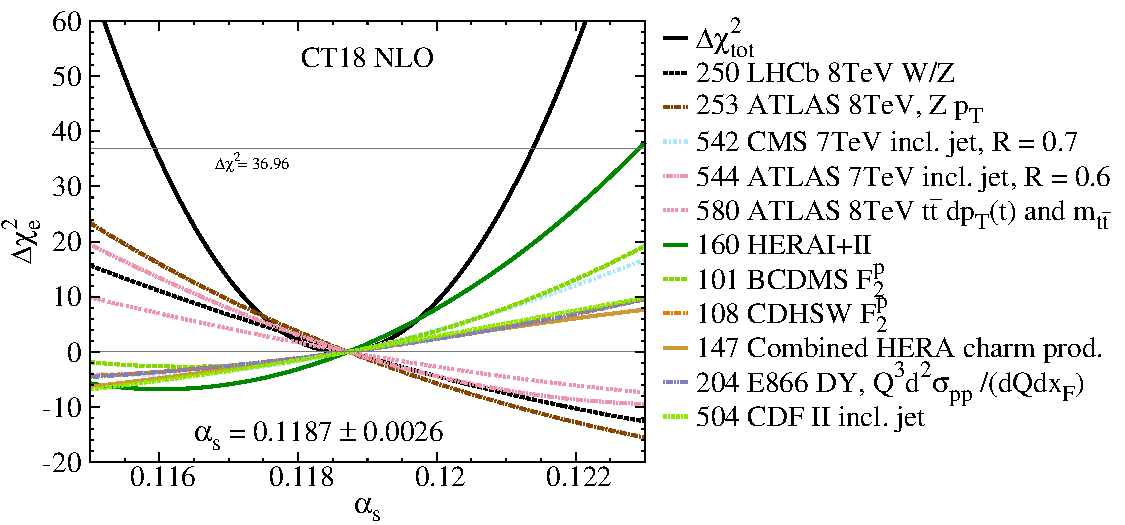
\includegraphics[width=0.8\textwidth]{./fig/LM/i2Tn2as0_11872_DEchi2_re2_ect.pdf}
\caption{
	Like Fig.~\ref{fig:lm_alphas}, but now showing the scan of $\alpha_s(M_Z)$ at NLO precision in $\alpha_s$.
        }
\label{fig:lm_alphas_nlo}
\end{figure}
%

From Fig.~\ref{fig:lm_alphas}, we see that the various data sets
have different sensitivities to both
the central  value of $\alpha_s(M_Z)$ and its uncertainty.  
According to the scans, the greatest sensitivity to $\alpha_s(M_Z)$ is provided by the HERA I+II data set, followed by the BCDMS proton data. Relatively to the full CT18 data set, both experiments prefer a lower value of
$\alpha_s(M_Z)$, on the order of $0.114-0.116$, but with wider uncertainties. The dependence of those two DIS data sets on $\alpha_s(M_Z)$ is primarily through the effect of scaling violation, but the sheer number of data points,
and the experimental and theoretical precision, lead to their large sensitivities. 

The LHC inclusive jet production, especially the CMS 7 and 8 TeV data, generally prefer a large value of $\alpha_s(M_Z)$, as
does the ATLAS 8 TeV Z $p_T$ data. The full CT18 data set prefers a value of $\alpha_s(M_Z, \mbox{NNLO})=0.1164 \pm 0.0026$, at 68\% C.L., defined using the ``global tolerance" prescription to correspond to a $\Delta \chi^2\! =\! 37$ interval
(the corresponding 90\% interval is defined by $\Delta \chi^2\! =\! 100$). The extracted value of $\alpha_s(M_Z)$ obtained with CT18Z is very similar, $0.1169\pm0.0026$, cf. Fig.~\ref{fig:lm_alphasz}. These values are to be
compared with $\alpha_s(M_Z)\!=\!0.1150^{+0.0036}_{-0.0024}$ as obtained by CT14 with a smaller HERA+LHC data set. 

The $\Delta\chi^2$ distribution for the full data set is very
parabolic, less so for the individual data sets. The $\Delta\chi^2$
curves for collections of data sets, for example, all DIS data, all DY
data, and all jets and top data, also appear parabolic, as expected
from the central limit theorem. From the right panel of
Fig.~\ref{fig:lm_alphas}, it is clear that the totality of DIS data
prefer a smaller value of $\alpha_s(M_Z)$  than the DY pair, jet and
top-quark production.  
The exact size of the $\alpha_s$ uncertainty thus is not well
determined and depends on the convention, as the pulls from various
(types of) experiments are not consistent at the level of few tens of
units of $\chi^2$.  

The scan exercise can also be carried out at NLO in $\alpha_s$, as we show in Fig.~\ref{fig:lm_alphas_nlo}. In fact, any difference between the NLO and NNLO results can serve as a partial estimate of the
theoretical uncertainty of its determination. Although the uncertainty is similar to that obtained at NNLO, the central value is slightly higher: $\alpha_s(M_Z,\mbox{NLO})=0.1187\pm 0.0027$. We note that the qualitative interplay of the experiments with leading sensitivity to $\alpha_s(M_Z)$ is much the same at NLO as
found at NNLO, with the combined HERA (Exp.~ID=160) and BCDMS $F^p_2$ data (Exp.~ID=101) again preferring lower values, while the ATLAS 7 TeV jet data (Exp.~ID=544) and 8 TeV
$Z$ $p_T$ data (Exp.~ID=253) pulling in the opposing direction, but more strongly at NLO than at NNLO. The preference of a higher $\alpha_s$ value at NLO by an amount of about 0.002 is consistent with findings of other PDF groups~\cite{Ball:2011us,Harland-Lang:2015nxa,Abramowicz:2015mha,Alekhin:2017kpj}.


To summarize, we find that the CT18 data set prefers a larger value of $\alpha_{s}(M_Z)$ and a marginally smaller nominal uncertainty than in CT14.


%
\begin{figure}[tbp]
\centering
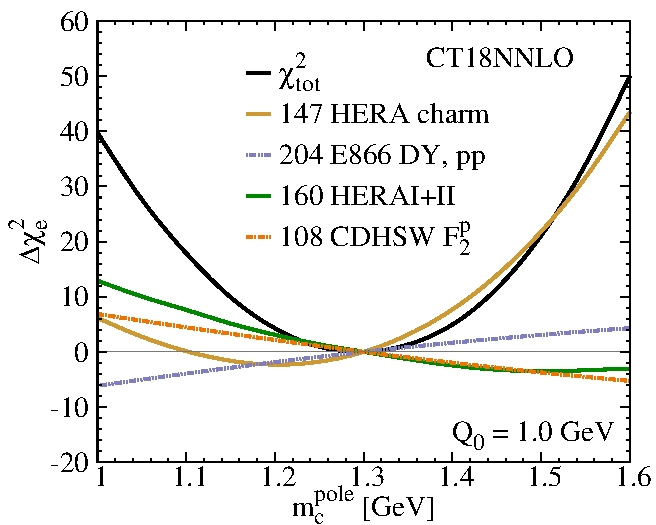
\includegraphics[width=0.6\textwidth]{./fig/LM/i2Tn3Q01-00mc1-30_DEchi2_re_ect.pdf}
\caption{
	A $\chi^2$ scan over values of the charm pole mass, $m_c$, at NNLO, using the CT18 data set. The settings of the fit are described in the text. The CT18Z counterpart to this $m_c$ scan is presented in Fig.~\ref{fig:lm_mcZ} in App.~\ref{sec:AppendixCT18Z}.
        }
\label{fig:lm_mc}
\end{figure}
%

{\bf Constraining the charm pole mass}.
Similar investigations can be carried out for other inputs of the perturbative theory, such as the pole mass of the charm
quark, $m_c$. A conclusive study on the charm mass dependence is beyond the scope of this article: the experimental preferences for $m_c$ may be affected by the initial scale $Q_0$, auxiliary settings in the heavy-quark scheme, and possibility of the nonperturbative charm \cite{Gao:2013wwa,Hou:2017khm,Dulat:2013hea}. In the candidate fits we made, we observe that the traditional choice $m_c^{pole}=1.3$ GeV remains compatible with the CT18(Z) global data, however, the most recent HERA DIS and LHC vector boson production experiments in totality may mildly prefer the pole mass of 1.4 GeV or higher. 

An illustration of the observed trends can be viewed in
Fig.~\ref{fig:lm_mc}, where we show the $\chi^2$ variation for the
total data set and for the leading experiments in a NNLO fit to the
CT18 data set at different pole $m_c$. To separate the $m_c$ dependence from $Q_0$ dependence, we set $Q_0=1$ GeV and use a more flexible gluon parametrization that better accommodates the full range of solutions at such low $Q$. 
As can be seen based on the minimum of the heavy black curve, the scan prefers a value of $m_c\! =\! 1.3$ GeV, with this mass
being somewhat larger than the preference of the combined charm production data from HERA (Exp.~ID=147) alone, which would otherwise suggest
$m_c\!\gtrsim\!1.2$ GeV. The combined HERA Run I and II inclusive data, on the other hand, essentially provide a lower bound to $m_c$, and prefer
a larger magnitude, $m_c\! > \!1.45$ GeV. 
However, these preferences are quite weak, yielding an overall change by ten units of $\chi^2$ over a large range of $m_c$.
The individual sensitivities of the other experiments presented in Fig.~\ref{fig:lm_mc} are even weaker.
It should be pointed out that the inclusion of the ATLAS 7 TeV $W$/$Z$ data (Exp.~ID=248) and other changes associated with CT18Z lead to a reconfiguration of the picture shown in Fig.~\ref{fig:lm_mc} and to an increase in the best-fit value of $m_c$, as we show in Fig.~\ref{fig:lm_mcZ} and discuss in App.~\ref{sec:AppendixCT18Z}.
In the same spirit, the patterns of the pulls change somewhat if we set $Q_0=m_c$ (another acceptable choice). 

% ~ ~ ~ ~ ~ ~ ~ ~ ~ ~ ~ ~ ~ ~ ~ ~ ~ ~ ~ ~ ~ ~ ~ ~ ~ ~ ~ ~ ~ ~ ~ ~ ~ ~

\subsection{Parton luminosities at the LHC
\label{sec:PDFLuminosities}
}

In Fig.~\ref{fig:lumia}, we show the parton luminosities
at the
LHC 14 TeV computed with the CT18 and CT18Z NNLO PDFs, contrasting them with
the previous \CTHERAII~release. To compare the luminosities only within the physically accessible regions, we compute the integrals of the luminosity with a restriction on the absolute rapidity of the final state to be
within 5 units, cf. Eq. (28) in \cite{Hou:2016sho}. In the comparisons for each
flavor combination, we again show results normalized either to a common reference 
(either CT18 NNLO or NLO) in the left-hand plots or to their respective central
predictions.

As in the case of individual PDFs, the CT18 central results for the parton
luminosities remain very close to \CTHERAII. On the other hand, the
PDF uncertainties of the luminosities for the individual PDF ensembles
are broadly reduced, especially for those 
luminosities involving gluons. In the region of the Higgs 
boson mass, $M_X\! \sim\! 125$ GeV, the improvement on the $gg$ luminosity, $L_\mathit{gg}$, shown
in the lowest panels of Fig.~\ref{fig:lumia}, is very small.
In the TeV-scale mass range, however, reductions in the PDF uncertainties of $L_\mathit{gg}$ are
more sizable, closer to $\sim\!20\%$.
%
Parton luminosities computed using CT18Z NNLO behave distinctly from CT18 in several respects. For example, in the
$W/Z$ boson-mass region, the central predictions for the $qq$ luminosity are approximately $3\!-\!4\%$
higher in CT18Z relative to CT18. The other parton luminosities are similarly enhanced in CT18Z
in the low-mass region, $M_X\! \lesssim\! 100$ GeV, in contrast to CT18, which more closely
resembles \CTHERAII.
%
While the high-mass quark-quark luminosity, $L_{qq}$, is relatively unmodified in CT18Z, 
$L_{gq}$ and $L_{gg}$ are suppressed for $M_X\! \gtrsim\! 100\!-\!300$ GeV; for the
gluon-gluon luminosity, this suppression can be as large as $\sim\!4\%$
between 100 GeV and 1 TeV. 

In Figs.~\ref{fig:lumiCT18NLOvsothers}
and~\ref{fig:lumiCT18NNLOvsothers}, we compare these
parton luminosities against those from other groups:
CJ15~\cite{Accardi:2016qay}, MMHT14~\cite{Harland-Lang:2014zoa}, and
NNPDF3.1~\cite{Ball:2017nwa}. Here we adopt the rescaled 68\% C.L. for
the CT18 PDFs to match the convention of the other groups. 
The comparison in Fig.~\ref{fig:lumiCT18NLOvsothers} is done at NLO, 
because CJ15 PDFs are not available at NNLO in QCD. 
The PDF uncertainties on the CJ15 NLO luminosities
are smaller than those on the CT18 NLO (see right insets), in part 
due to a smaller tolerance criterion ($\Delta \chi^2 =1$) and less
flexible parametrization forms for the $\bar u$ and $\bar d$ PDFs
employed by CJ15.
The CT18 NLO $qq$ luminosity central value is approximately 8\% to 5\% higher than CJ15 for mass 
values $10\lesssim M_{X}\lesssim 2\cdot  10^{3}$ GeV and up to 8-10\% lower for higher values (see left insets). 
The CT18 PDF error band for $L_{qq}$ covers that of CJ15  over the mass range $20\lesssim M_{X}\lesssim 2\cdot  10^{3}$ GeV. 
The CT18 NLO $gq$ luminosity is approximately 2\% higher than CJ15 in
the mass region relevant for Higgs production,
$100\lesssim M_{X}\lesssim 300$ GeV. It is also higher everywhere
else,  
with major differences present
at low masses, $M_X\lesssim 100$ GeV, where it is 8\% higher,
and at high masses, $M_X \gtrsim 650$ GeV, where differences are about 12\% at $M_X \approx 5$ TeV. 
For the $gg$ luminosity, CT18 at NLO is higher everywhere, in particular, differences are larger than 20\% at $M_X \approx 5$ TeV.

The luminosities obtained using CT18 NNLO PDFs are compared to those obtained with MMHT14 and NNPDF3.1 PDFs in Fig.~\ref{fig:lumiCT18NNLOvsothers}. 
The NNPDF3.1 PDFs set is selected with $\alpha_s(M_Z) = 0.118$. 
The  central values  of $qq$ and $gq$ luminosities for the three
groups agree within a few percent in the mass region $100\lesssim
M_{X}\lesssim 10^{3}$ GeV, where they also have comparable PDF
uncertainties. The CT18 NNLO $gg$ luminosity is approximately 2\%
smaller than both NNPDF3.1 and MMHT14 in the mass range
$20\lesssim M_{X}\lesssim 300$ GeV.
At larger masses $M_X \gtrsim 300$ GeV, we observe a rapid drop of the
NNPDF3.1 luminosity. Moreover, the NNPDF3.1 uncertainty is smaller
over all the mass range.      

 

\begin{widetext}

%FIGURE
\begin{figure}[!htbp]
	\begin{center}
		\hspace*{-0.4cm}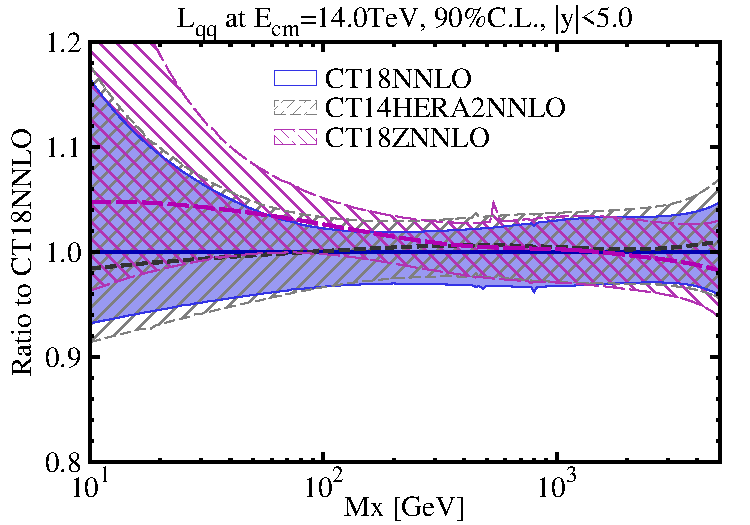
\includegraphics[width=0.48\textwidth]{./fig/qq_CT18.pdf}
		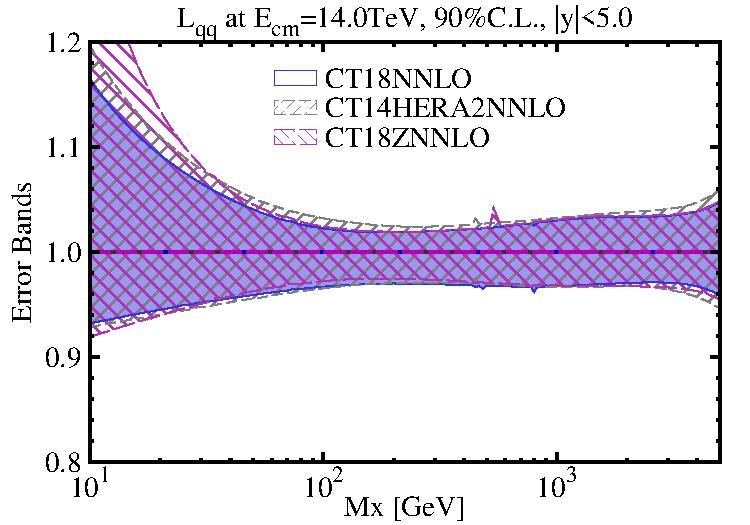
\includegraphics[width=0.48\textwidth]{./fig/qq_CT18_err.pdf} \\
		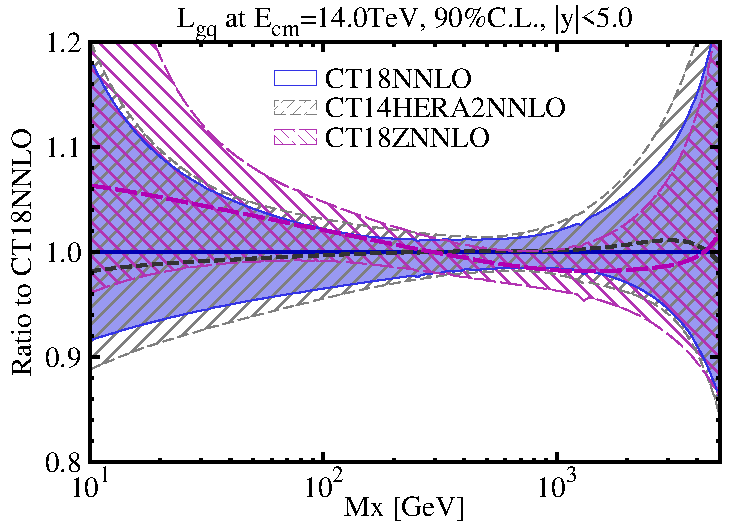
\includegraphics[width=0.48\textwidth]{./fig/gq_CT18.pdf}
		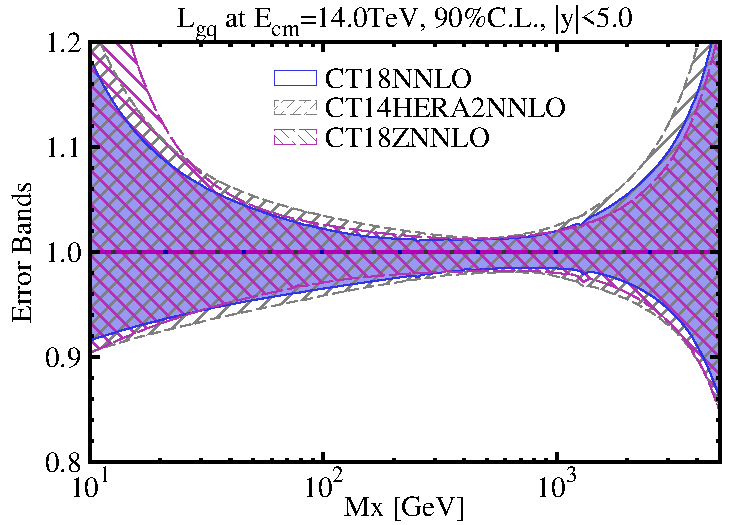
\includegraphics[width=0.48\textwidth]{./fig/gq_CT18_err.pdf} \\
		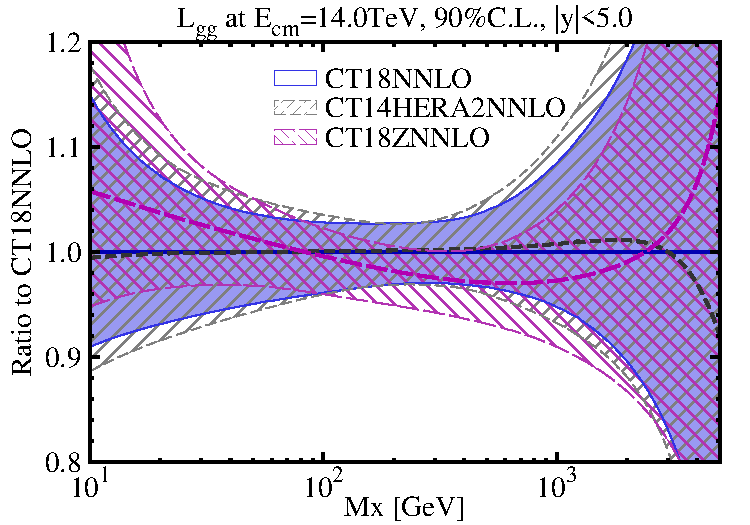
\includegraphics[width=0.48\textwidth]{./fig/gg_CT18.pdf}
		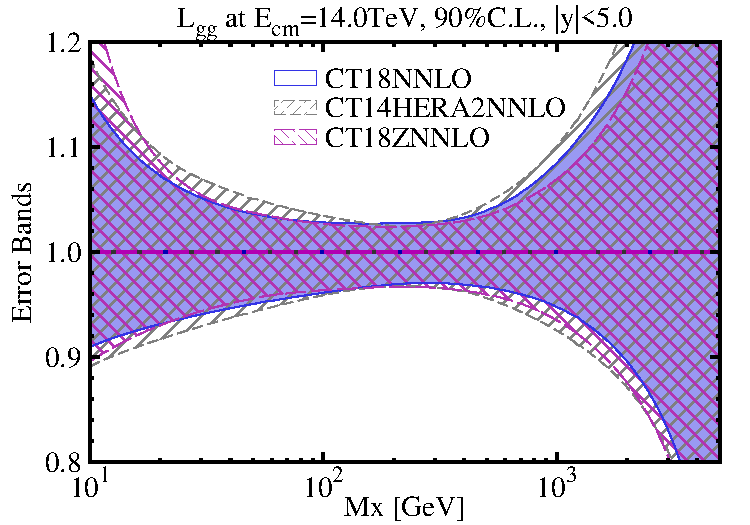
\includegraphics[width=0.48\textwidth]{./fig/gg_CT18_err.pdf}
	\end{center}
	\vspace{-2ex}
	\caption{
		%
		Parton luminosities for processes
		at the LHC at $\sqrt{s} = 14$ TeV, in the central
                rapidity region $|y|<5$: $L_{qq}$ (upper panels), $L_{gq}$ (center panels),
		and $L_{gg}$ (lower panels); evaluated using CT18 (solid violet), CT18Z (short-dashed
		gray), and CT14$_\mathrm{HERAII}$ (long-dashed magenta) NNLO PDFs. The left panels give
		the luminosity ratios normalized to CT18, whereas the right panels show the error bands for
		each luminosity, normalized for each PDF ensemble to
                its own central prediction. 
	}
\label{fig:lumia}
\end{figure}

\end{widetext}

%FIGURE
\begin{figure}[!htbp]
	\begin{center}
		\hspace*{-0.4cm}
		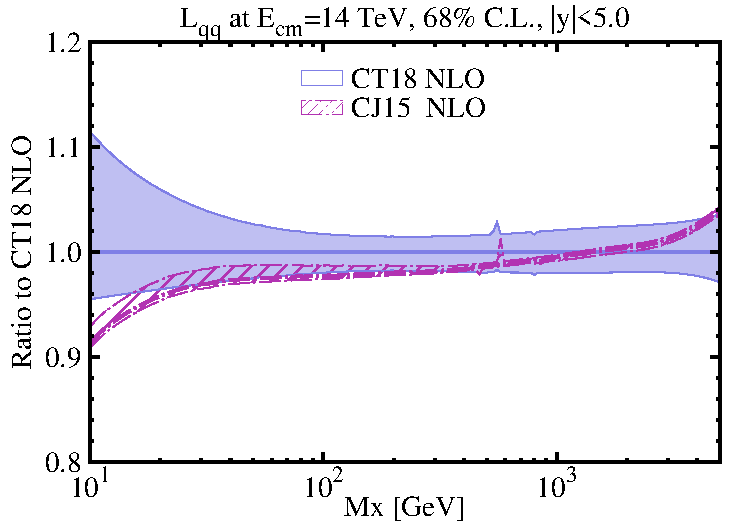
\includegraphics[width=0.48\textwidth]{./fig/Lumi_CT18NLO_CJ15nlo/Lumi_14TeV_ym-lt-5-0_asym_20__68CL-CT18NLO_CJ15nlo__00_qQr_ect.pdf} 
		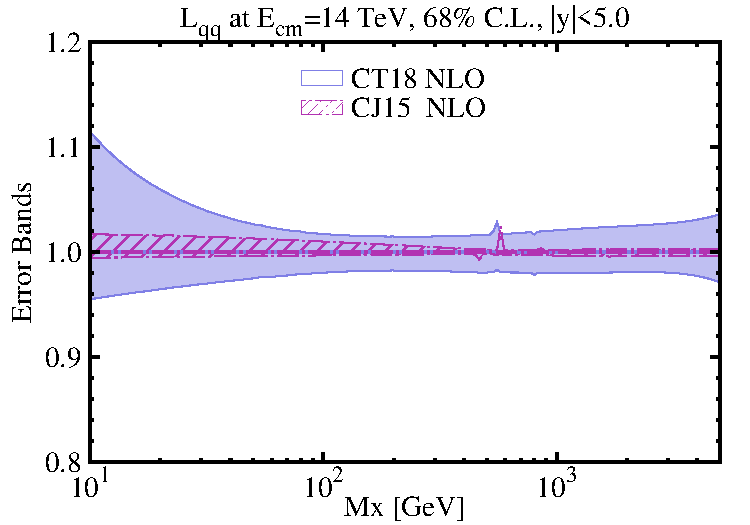
\includegraphics[width=0.48\textwidth]{./fig/Lumi_CT18NLO_CJ15nlo/Lumi_14TeV_ym-lt-5-0_asym_20__68CL-CT18NLO_CJ15nlo__00_qQ2_ect.pdf} \\
		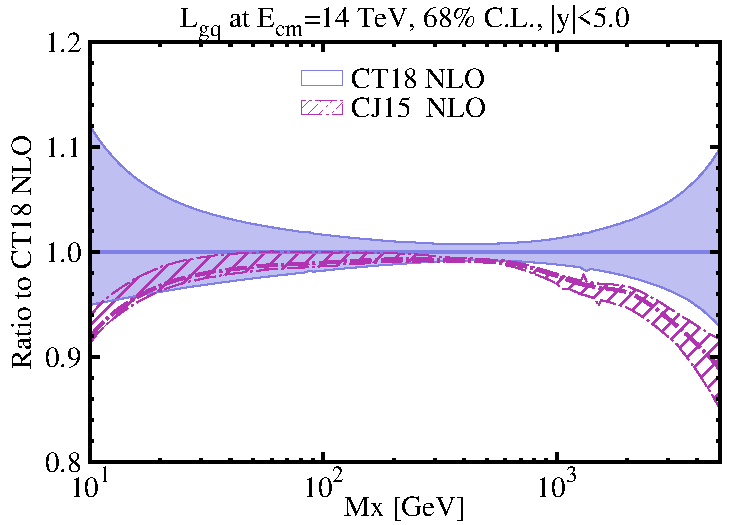
\includegraphics[width=0.48\textwidth]{./fig/Lumi_CT18NLO_CJ15nlo/Lumi_14TeV_ym-lt-5-0_asym_20__68CL-CT18NLO_CJ15nlo__00_gqr_ect.pdf} 
		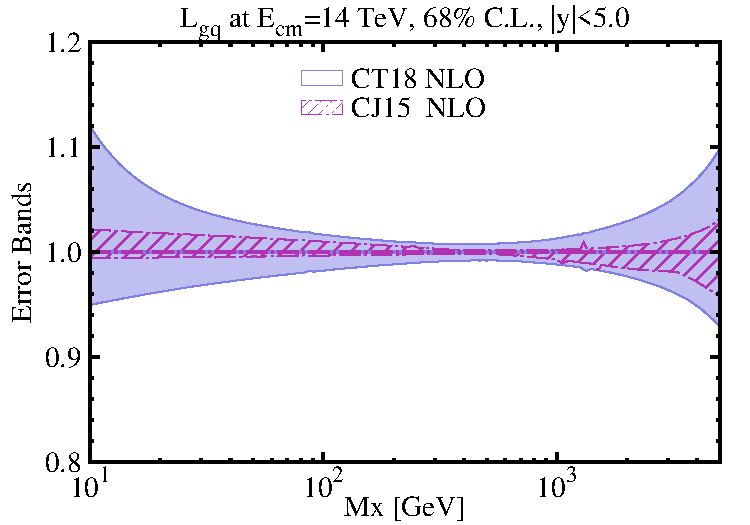
\includegraphics[width=0.48\textwidth]{./fig/Lumi_CT18NLO_CJ15nlo/Lumi_14TeV_ym-lt-5-0_asym_20__68CL-CT18NLO_CJ15nlo__00_gq2_ect.pdf} \\
		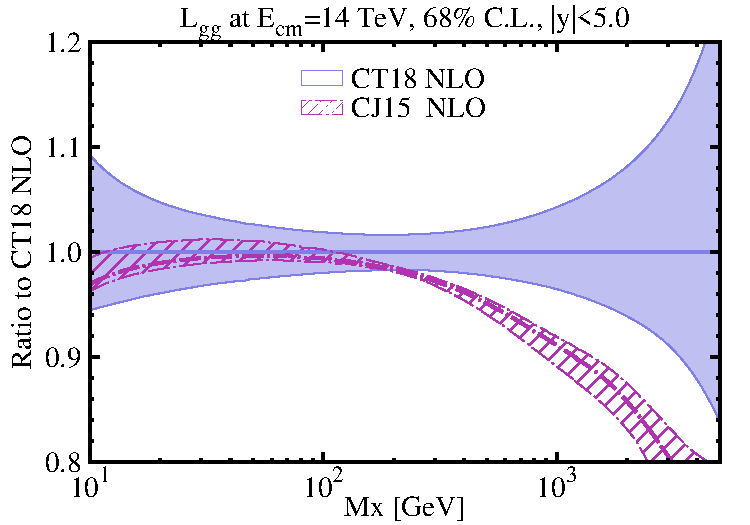
\includegraphics[width=0.48\textwidth]{./fig/Lumi_CT18NLO_CJ15nlo/Lumi_14TeV_ym-lt-5-0_asym_20__68CL-CT18NLO_CJ15nlo__00_ggr_ect.pdf}
		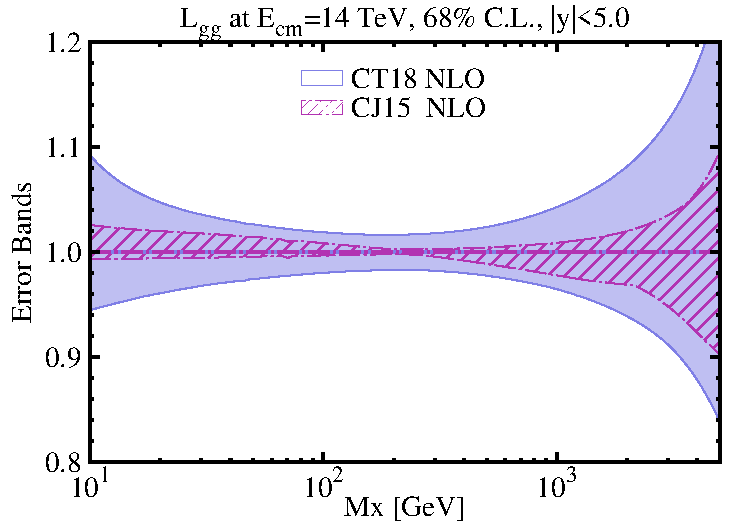
\includegraphics[width=0.48\textwidth]{./fig/Lumi_CT18NLO_CJ15nlo/Lumi_14TeV_ym-lt-5-0_asym_20__68CL-CT18NLO_CJ15nlo__00_gg2_ect.pdf}

	\end{center}
	\vspace{-2ex}
	\caption{Same as Fig.~\ref{fig:lumia}, comparing the CT18 NLO and CJ15 NLO parton luminosities.
	}
\label{fig:lumiCT18NLOvsothers}
\end{figure}

\clearpage

% 
\begin{figure}[!htbp]
	\begin{center}
		\hspace*{-0.4cm}
		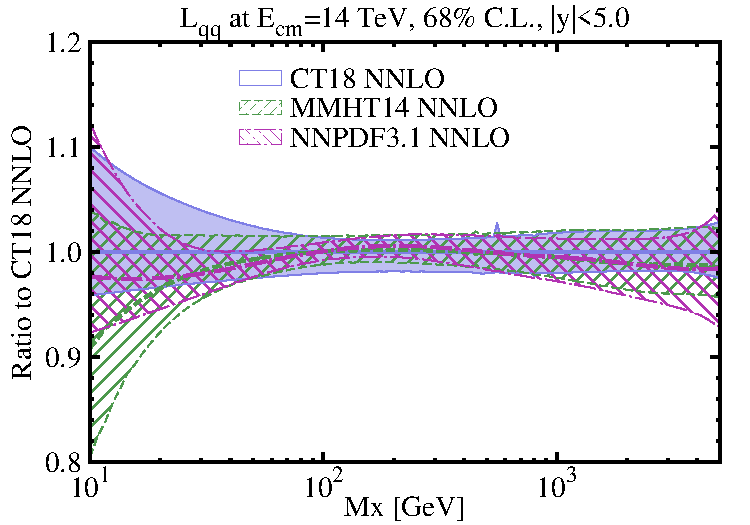
\includegraphics[width=0.48\textwidth]{./fig/Lumi_CT18NNLO_MMHT_NNPDF31/Lumi_14TeV_ym-lt-5-0_asym_30__68CL-CT18NNLO_MMHT2014nnlo_NNPDF31nnloas01181000__00_qQr_ect.pdf} 
		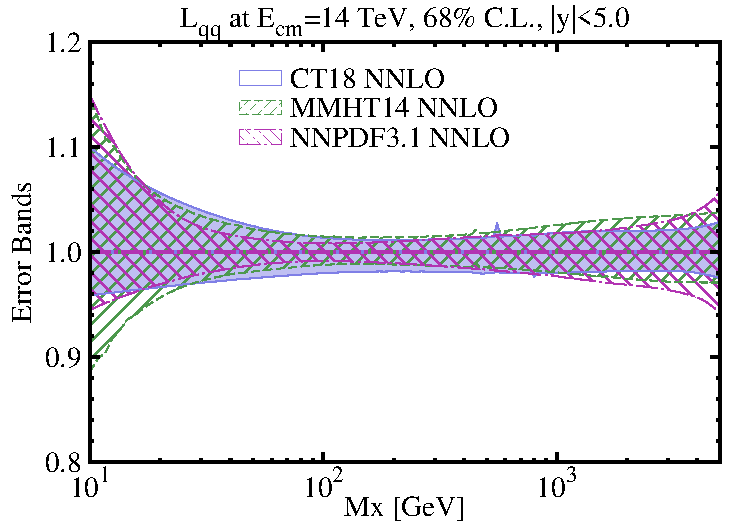
\includegraphics[width=0.48\textwidth]{./fig/Lumi_CT18NNLO_MMHT_NNPDF31/Lumi_14TeV_ym-lt-5-0_asym_30__68CL-CT18NNLO_MMHT2014nnlo_NNPDF31nnloas01181000__00_qQ2_ect.pdf} \\
		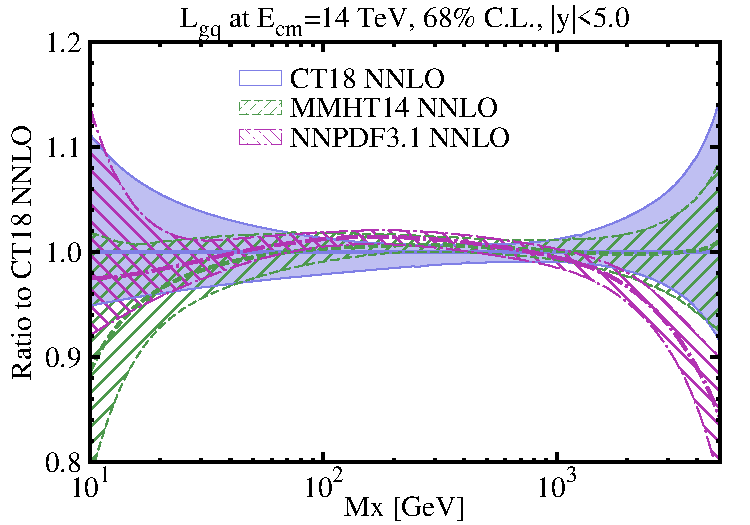
\includegraphics[width=0.48\textwidth]{./fig/Lumi_CT18NNLO_MMHT_NNPDF31/Lumi_14TeV_ym-lt-5-0_asym_30__68CL-CT18NNLO_MMHT2014nnlo_NNPDF31nnloas01181000__00_gqr_ect.pdf} 
		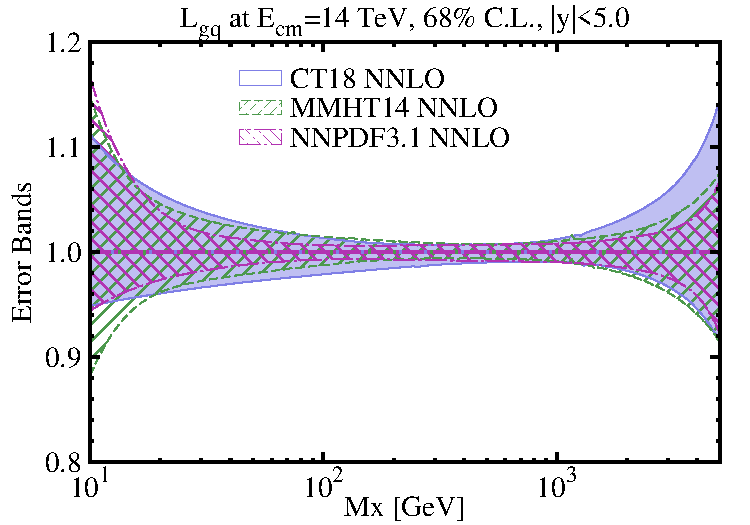
\includegraphics[width=0.48\textwidth]{./fig/Lumi_CT18NNLO_MMHT_NNPDF31/Lumi_14TeV_ym-lt-5-0_asym_30__68CL-CT18NNLO_MMHT2014nnlo_NNPDF31nnloas01181000__00_gq2_ect.pdf} \\
		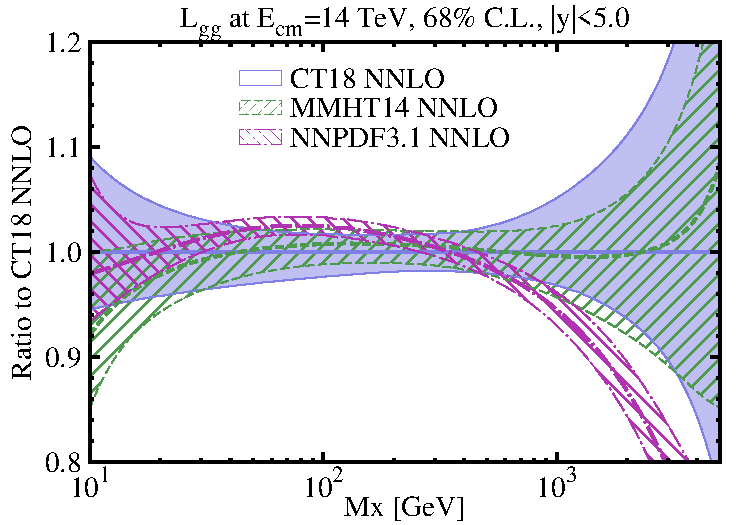
\includegraphics[width=0.48\textwidth]{./fig/Lumi_CT18NNLO_MMHT_NNPDF31/Lumi_14TeV_ym-lt-5-0_asym_30__68CL-CT18NNLO_MMHT2014nnlo_NNPDF31nnloas01181000__00_ggr_ect.pdf}
		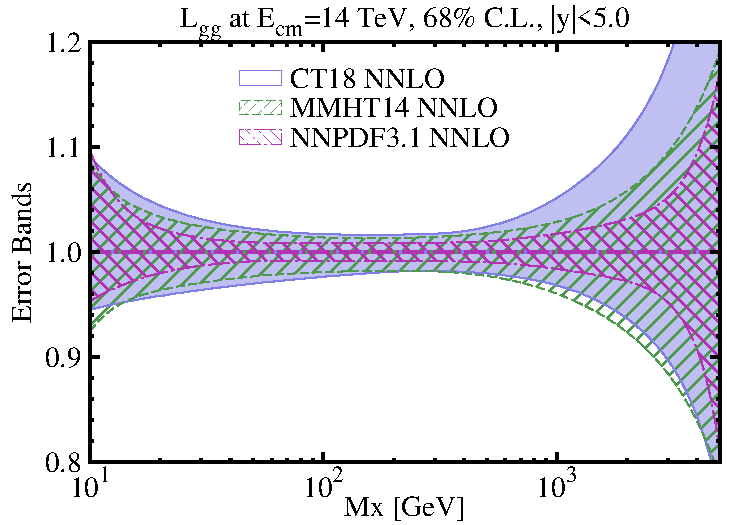
\includegraphics[width=0.48\textwidth]{./fig/Lumi_CT18NNLO_MMHT_NNPDF31/Lumi_14TeV_ym-lt-5-0_asym_30__68CL-CT18NNLO_MMHT2014nnlo_NNPDF31nnloas01181000__00_gg2_ect.pdf}

	\end{center}
	\vspace{-2ex}
	\caption{Same as Fig.~\ref{fig:lumia}, comparing the CT18,
          MMHT'2014, and NNPDF3.1 NNLO parton luminosities with
          $\alpha_s(M_Z)=0.118$.  
	}
\label{fig:lumiCT18NNLOvsothers}
\end{figure}


\clearpage


% - - - - - - - -
%
\subsection{PDF moments and sum rules}
\label{sec:moments}
%
%\NOTE{Draft of this section by Tim.}
%A summary of main results has been included, three new
%figures uploaded. A new table with a comparison to lattice results and associated refs has been added. Revised
%to include a discussion of the lattice comparisons.}
%


Knowledge of the integrated PDF {\it Mellin} moments has long been of interest, both for their phenomenological
utility, and for their relevance to lattice QCD computations of hadronic structure \cite{Lin:2017snn,Hobbs:2019gob}.
In the case of the former, PDF moments can serve as valuable benchmarks for the purpose of comparing various global
analyses and theoretical approaches, and can also be informative descriptors of the PDFs themselves. This follows
especially from the fact that numerical results obtained for PDFs of a given order are connected with the $x$
dependence of the underlying parton distribution, with, in general, higher-order Mellin moments mostly determined
by the PDFs' high-$x$ behavior.  In Ref.~\cite{Hobbs:2019gob}, an analysis of the sensitivities of HEP data to
lattice-calculable quantities --- specifically, the Mellin moments and parton quasi-distribution functions --- was
performed to further develop the still-emerging PDF-Lattice community effort \cite{Lin:2017snn}. 
%

Integrated moments can in general be evaluated for practically any phenomenological PDF from its underlying distribution,
provided the moment in question is convergent over the full range of support. However, in this analysis we concentrate
special attention on
%
\begin{equation}
\langle x^n\rangle_g(Q)=\int_{0}^{1}dx\ x^{n}\,  g(x,\Q) \, ,
\label{eq:gmom}
\end{equation}
%
with $n\!=\!1$ for the gluon, as well as
%
\begin{align}
	\langle x^n\rangle_{q^+}(Q) &= \int_{0}^{1}dx\ x^{n}\,  [q + \overline{q}](x,\Q) \ \ \mathrm{for}\ \ n = 1, 3, \dots \nonumber \\
%
	\langle x^n\rangle_{q^-}(Q) &= \int_{0}^{1}dx\ x^{n}\,  [q - \overline{q}](x,\Q) \ \ \mathrm{for}\ \ n = 2, 4, \dots
\label{eq:qmom}
\end{align}
%
for the quark distributions, where we denote the charge conjugation-even (odd) quark combinations as $q^\pm = q \pm \overline{q}$.
%	
We primarily consider these specific PDF moments of Eq.~(\ref{eq:gmom}) with $n\!=\!1$ and Eq.~(\ref{eq:qmom}) for compatibility with lattice QCD determinations,
which are only able to compute the odd ($n\! =\! 1, 3, \dots$) moments of $q\!+\!\bar{q}$-type distributions and even ($n\! =\! 2, 4, \dots$) moments
for $q\!-\!\bar{q}$-type distributions.
%
This follows from the fact that lattice calculations extract the integrated Mellin moments from hadronic matrix elements as,
%
%
\begin{equation}
	\frac{1}{2}\sum_{s}\langle p,s|\mathcal{O}_{\{\mu_{1},\cdots,\mu_{n+1}\}}^{q}|p,s\rangle = 2 \langle x^{n+1} \rangle_{q}\,[p_{\mu_{1}}\cdots p_{\mu_{n+1}}-{\rm traces}]\ .
\label{eq:OPE}
\end{equation}
%
%
In Eq.~(\ref{eq:OPE}), the lattice operators are
$\mathcal{O}_{\{\mu_{1},\cdots,\mu_{n+1}\}}\! \sim\! i^n \overline{q} \gamma_{\mu_1} \overleftrightarrow{D}_{\mu_2} \cdots \overleftrightarrow{D}_{\mu_{n+1}} q$, involving
covariant derivatives in such a way that successive derivative insertions increase the order of the extracted moment, but also alternate the even-/oddness under charge conjugation.


\begin{table}
%\vspace{-0.5cm}
%\hspace*{-1.3cm}\begin{tabular*}{\textwidth}{c| @{\extracolsep{\fill}} cc|c|ccc}
\begin{tabular*}{\textwidth}{c| @{\extracolsep{\fill}} cc|c|ccc}
\hline
PDF moment                             &   {\bf CT18}    &    {\bf CT18Z}   &    {\bf \CTHERAII}   &  {\bf MMHT14}   &   {\bf CJ15}      &     {\bf NNPDF3.1}    \tabularnewline
\hline                                                                                                                                                        
$\langle x \rangle_{u^+-d^+}$          &  $0.156(7)$     &    $0.156(6)$    &    $0.159(6)$     &   $0.151(4)$    &    $0.1518(13)$   &   $0.152(3)$          \tabularnewline
$\langle x^2 \rangle_{u^--d^-}$        &  $0.055(2)$     &    $0.055(2)$    &    $0.055(2)$     &   $0.053(2)$    &    $0.0548(2)$    &   $0.057(3)$          \tabularnewline
$\langle x^3 \rangle_{u^+-d^+}$        &  $0.022(1)$     &    $0.022(1)$    &    $0.022(1)$     &   $0.022(1)$    &    $0.0229(1)$    &   $0.022(1)$          \tabularnewline
\hline                                                                                                                                                        
$\langle x \rangle_{g}$                &  $0.414(8)$     &    $0.407(8)$    &    $0.415(8)$     &   $0.411(9)$    &    $0.4162(8)$    &   $0.410(4)$          \tabularnewline
\hline                                                                                                                                                        
$\langle x \rangle_{u^+}$              &  $0.350(5)$     &    $0.350(4)$    &    $0.351(5)$     &   $0.348(5)$    &    $0.3480(6)$    &   $0.348(4)$          \tabularnewline
$\langle x \rangle_{d^+}$              &  $0.193(5)$     &    $0.194(5)$    &    $0.193(6)$     &   $0.197(5)$    &    $0.1962(9)$    &   $0.196(4)$          \tabularnewline
$\langle x \rangle_{s^+}$              &  $0.033(9)$     &    $0.041(8)$    &    $0.031(8)$     &   $0.035(8)$    &    $0.0313(2)$    &   $0.039(4)$          \tabularnewline
\hline                                                                                                                                                        
$\langle x^2 \rangle_{u^-}$            &  $0.085(1)$     &    $0.084(1)$    &    $0.085(1)$     &   $0.083(1)$    &    $0.0853(2)$    &   $0.085(3)$          \tabularnewline
$\langle x^2 \rangle_{d^-}$            &  $0.030(1)$     &    $0.029(1)$    &    $0.030(1)$     &   $0.030(1)$    &    $0.0305(2)$    &   $0.028(3)$          \tabularnewline
$\langle x^2 \rangle_{s^-}$            &    ---          &      ---         &      ---          &   $0.001(1)$    &      ---          &   $0.001(4)$          \tabularnewline
\hline                                                                                                                                                        
$\langle 1 \rangle_{\bar{d}-\bar{u}}$  &  $-0.12(35)$    &    $-0.07(29)$   &    $-0.37(41)$    &   $0.084(15)$   &    $0.103(20)$    &     ---               \tabularnewline
$\kappa_s$                             &  $0.49(16)$     &    $0.61(14)$    &    $0.46(13)$     &   $0.51(14)$    &      ---          &   $0.563(82)$         \tabularnewline
%
%
%
\end{tabular*}\caption{
	We collect values of several PDF moments computed according to CT18, CT18Z, CT14$_\mathrm{HERAII}$, MMHT14, CJ15 NLO, and
	NNPDF3.1, all at the scale $Q=2$ GeV. The moments are chosen for their dual interest both as benchmarks for phenomenological calculations and relevance
	to lattice QCD calculations. In the descending order, we show the three lowest moments of the isovector ($u\!-\!d$) distribution, the first
	moment of the gluon, the first and second moments, respectively, for the flavor-separated $u, d, s$ distributions, and two measures
	of light quark flavor symmetry violation: the zeroth moment of the flavor $\mathrm{SU}(2)$ difference, $\langle 1 \rangle_{\bar{d}-\bar{u}}$,
	and the moment ratio related to the strangeness suppression, $\kappa_s$, defined in Eq.~(\ref{eq:str-supp}). We note that the $\bar{d}$ and
	$\bar{u}$ distributions are not constrained to coincide at $x\!\to\!0$ in NNPDF3.1, leaving $\langle 1 \rangle_{\bar{d}-\bar{u}}$ undefined,
	whereas the strange suppression factor was not fitted in CJ15.  Here, all computed moment uncertainties are either based on 68\% C.L., or have been rescaled accordingly for comparison.
}
\label{tab:moments}
\end{table}
%
%

%

\begin{figure*}
%\hspace{-.75cm}
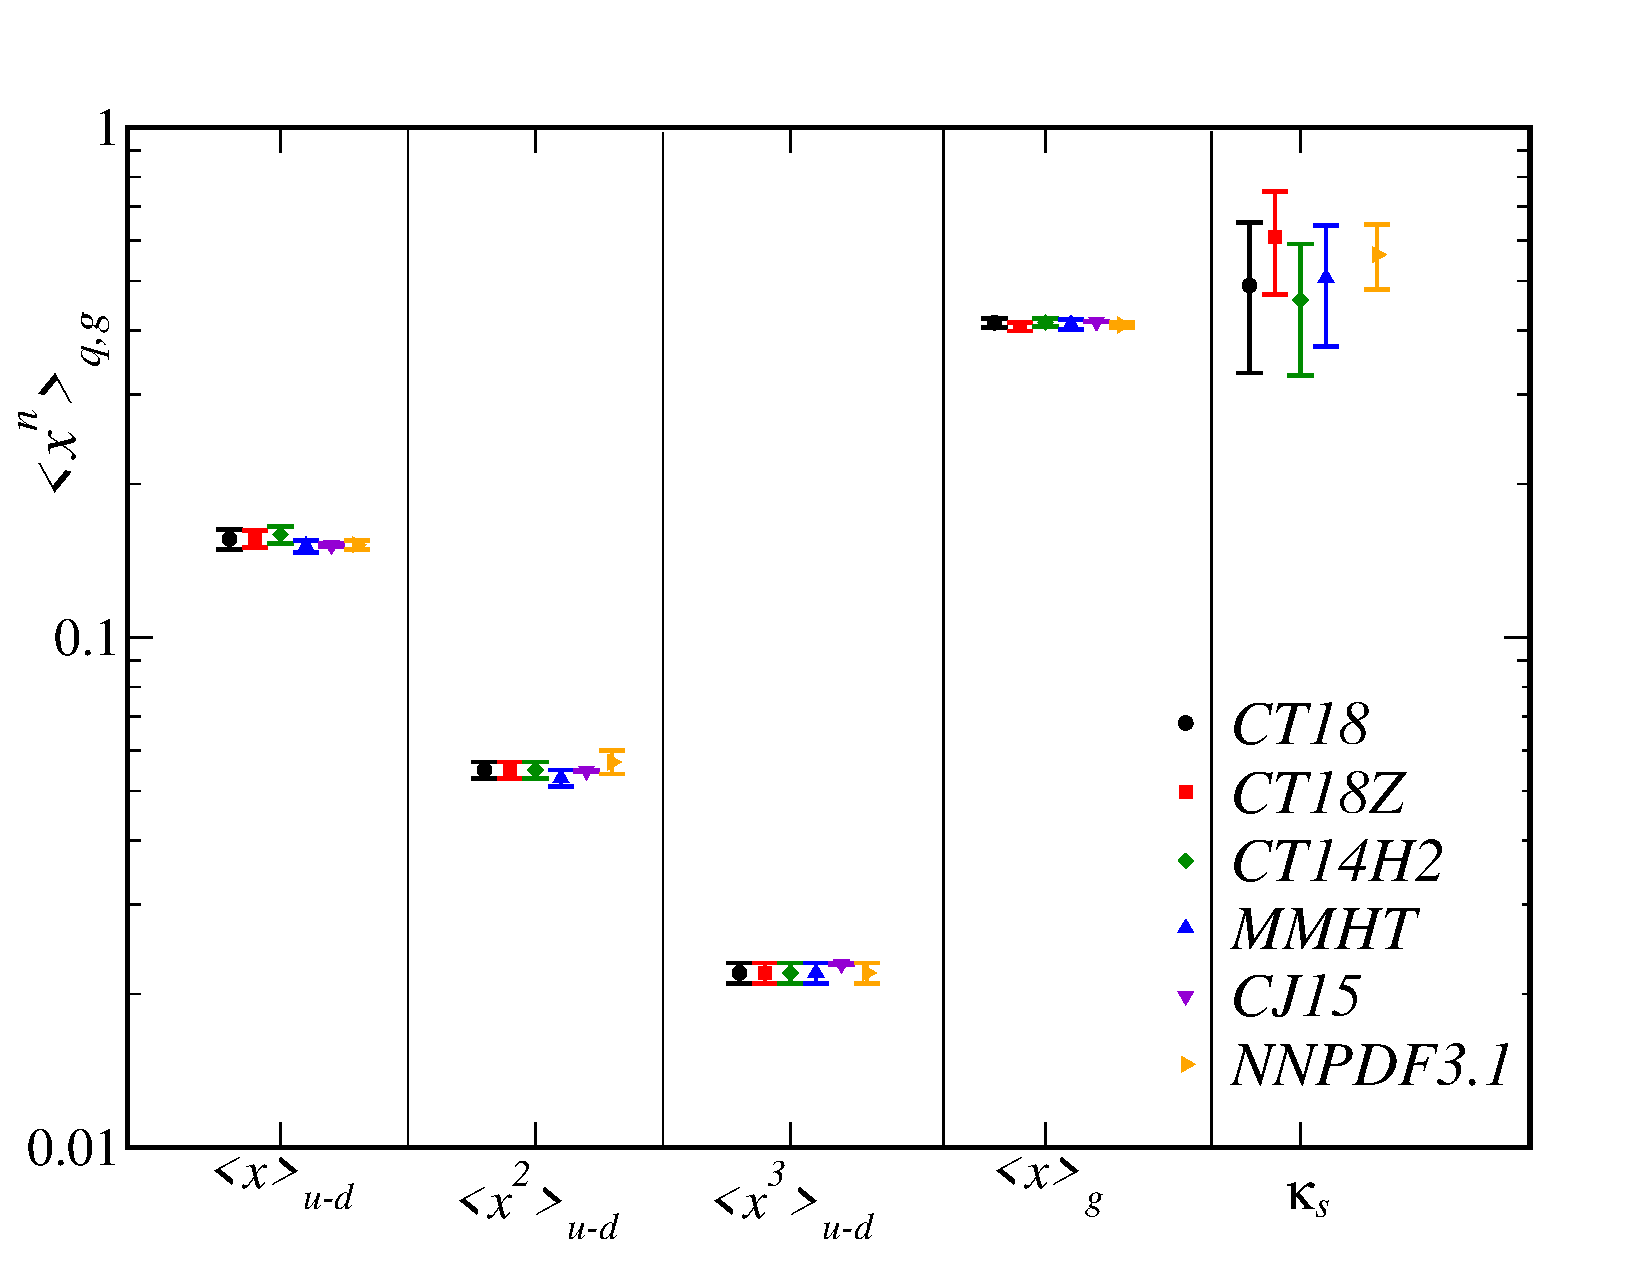
\includegraphics[scale=0.29]{./fig/mom-comps_v3.pdf}
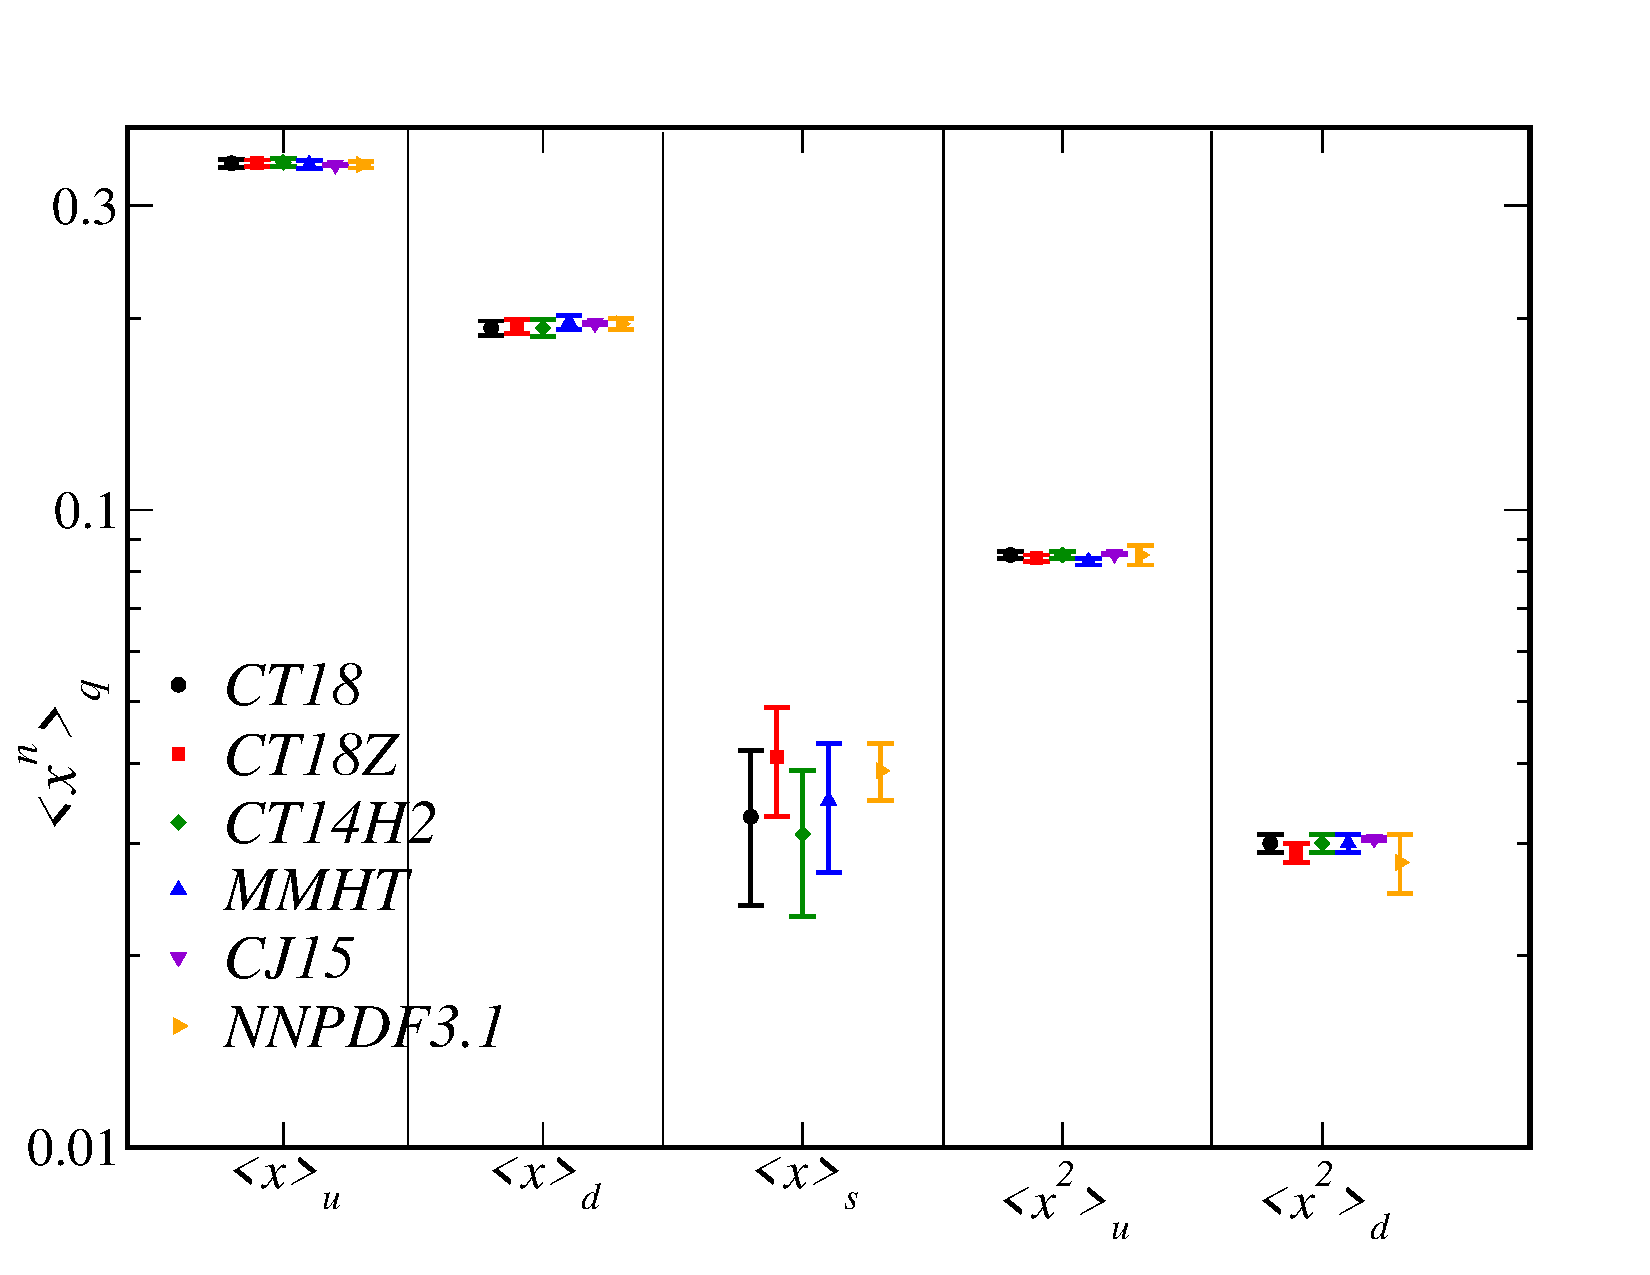
\includegraphics[scale=0.29]{./fig/mom-comps_FS_v2.pdf}
%
\caption{
	A graphical comparison of the PDF moments summarized in Table~\ref{tab:moments}, with the exception of the
	results for the zeroth moment of $\bar{d}-\bar{u}$ combination, relevant for studies of the
	Gottfried Sum Rule; this latter quantity is given in
        Fig.~\ref{fig:moments2}. The CJ15 global fit does not
        determine $\kappa_s$ and $\langle x \rangle_{s}$ as
        independent entities from the data, their respective
        predictions are not shown. 
}
\label{fig:moments1}
\end{figure*}
%


%
\begin{figure*}
%	\vspace{-1.75cm}
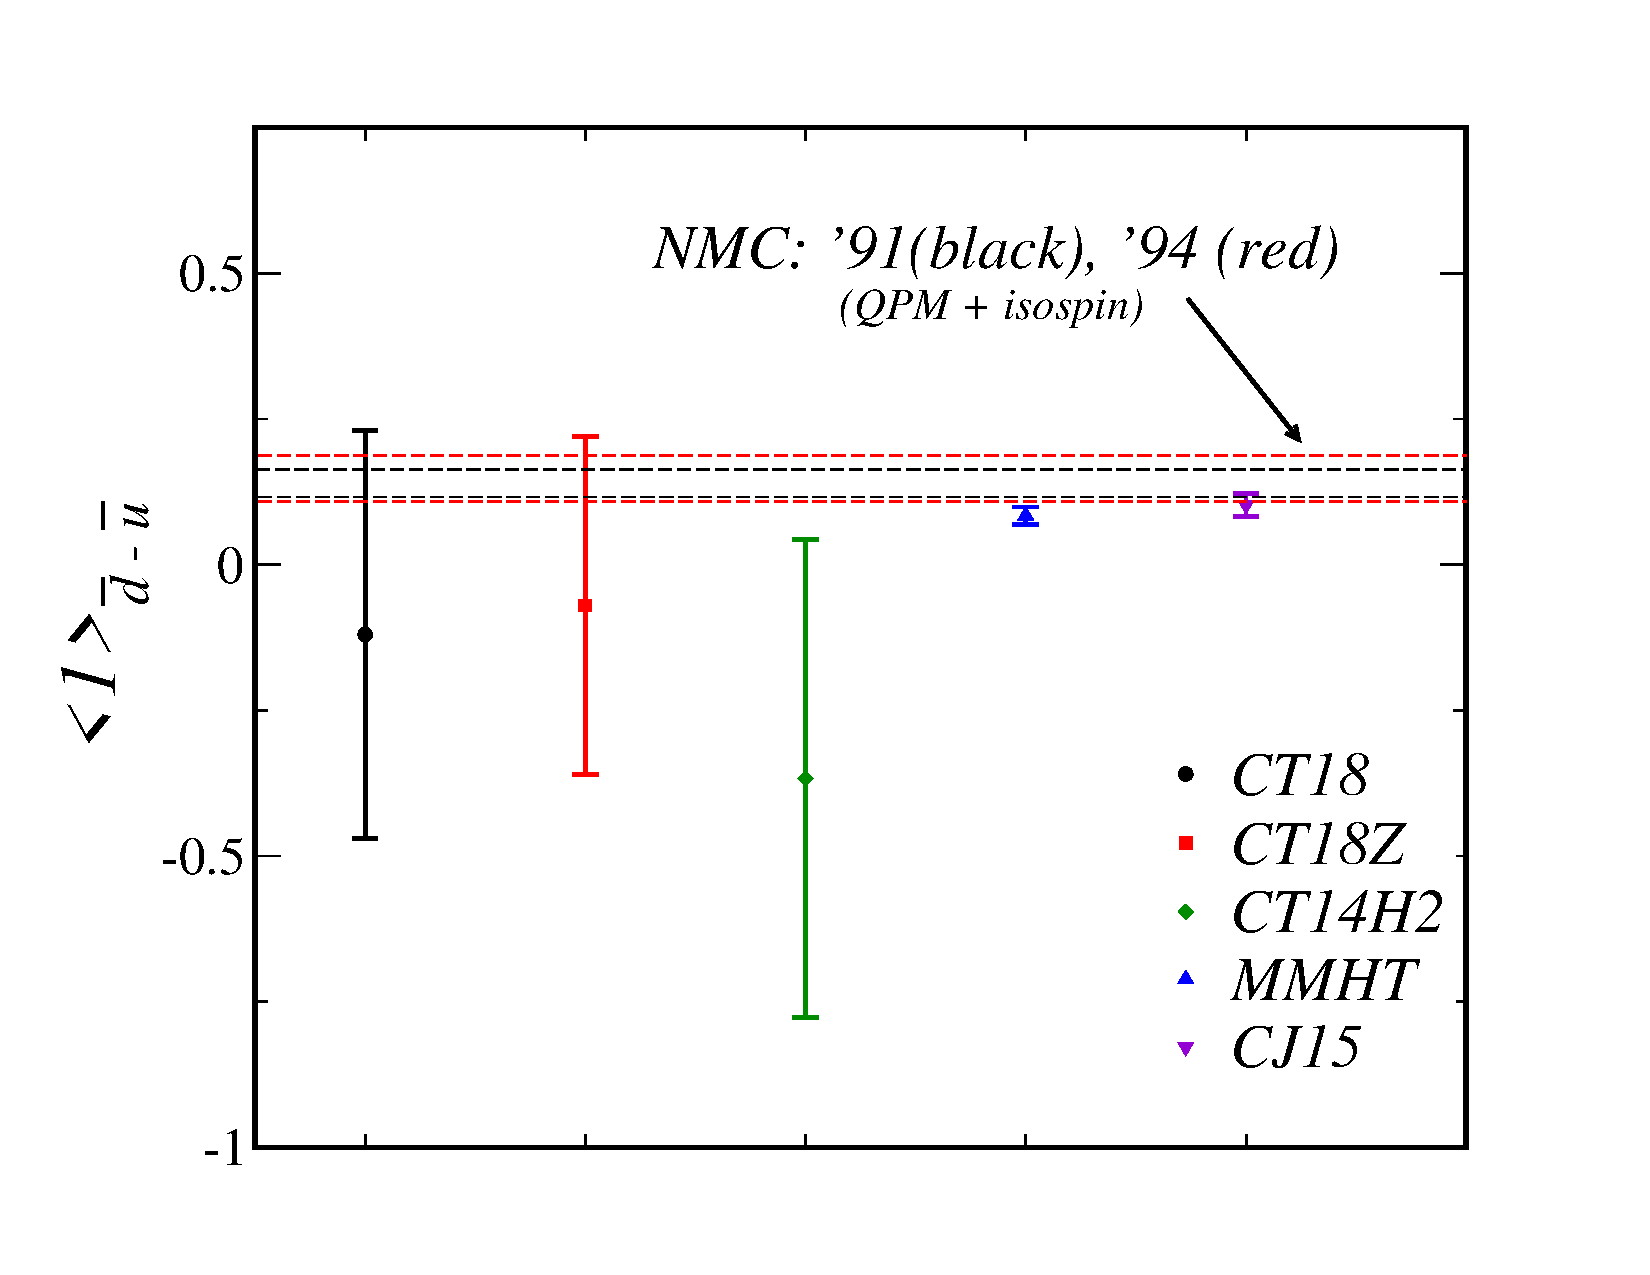
\includegraphics[scale=0.45]{./fig/Gott-comps_v3.pdf}
%
	\vspace{-1.1cm}
\caption{
	A visual comparison of the results for $\int_0^1 dx [\bar{d}(x)-\bar{u}(x)]$. The horizontal
	nested black and red bands correspond to the values extracted from the original NMC analyses from 1991~\cite{Amaudruz:1991at} and 1994~\cite{Arneodo:1994sh}, respectively. These were based on direct
	quark-parton model extractions of the flavor asymmetry PDF from the deuteron-to-proton
	structure function ratio measured at $Q^2 = 4$ GeV$^2$ for a range of $x \lesssim 0.7$. While
	all but the highest $x$ bin in this data set is consistent with CTEQ kinematical cuts,
	the very low $Q$ is exactly at the boundary of the $Q$ cut,
        and likely subject to substantial higher-twist corrections, especially for the higher $x$ bins.
}
\label{fig:moments2}
\end{figure*}
%

%
We compute a number of the typical benchmark PDF Mellin moments using our updated CT18 and CT18Z NNLO fits and compare against
the older CT14$_\mathrm{HERAII}$ NNLO parametrization as well as the recent MMHT14 NNLO, CJ15 NLO, and NNPDF3.1 global analyses.
In all cases, moments are evaluated for an $\overline{\mathrm{MS}}$ factorization scale of $\Q = 2$ GeV, which is also the
standard matching scale computed in lattice QCD calculations. We summarize the numerical results of the PDF moment calculations
in the entries of Table~\ref{tab:moments} as well as in Figs.~\ref{fig:moments1}--\ref{fig:moments2}.
%
We point out that the comparatively small values of the CJ15 NLO uncertainties are primarily attributable to the use of
$\Delta \chi^2 = 1$ criterion, and, in some cases, a comparatively more restrictive parametrization.

%
%
%-   -   -    -    -    -    -    -    -    -    -    -   -   -    -    -    -    -    -    -    -    -    -    -   -   -    -    -    -    -    -    -    -    -
%

{\it Observations.} In general, we observe concordance among the moments of the light distributions, including those of the isovector
({\it i.e.}, $u\!-\!d$) combination, $\langle x^{1,3} \rangle_{u^+-d^+}$ and $\langle x^2 \rangle_{u^--d^-}$. Notably, the CT results for the first isovector
moment, $\langle x \rangle_{u^+-d^+}\! \sim\! 0.156\!-\!0.159$, are marginally larger than those obtained under the other fits considered
here, which produce $\langle x \rangle_{u^+-d^+}\! \sim\! 0.151\!-\!0.152$, but are nevertheless in close agreement at the 1$\sigma$ level.
%
%
Similarly, we recover very robust agreement for the first moment of the gluon PDF, which can be understood to carry $\sim\! 41\%$
of the proton's longitudinal momentum at the scale $\Q = 2$ GeV. We find a slightly smaller total contribution
to the momentum sum rule from the gluon under CT18Z NNLO, which results in $\langle x \rangle_{g} = 0.407(8)$, in agreement with the default
CT18 NNLO calculation, $\langle x \rangle_{g} = 0.414(8)$. This is consistent with the modest reduction in the central
gluon shown for CT18Z in the lower-right panel of Fig.~\ref{fig:PDFbands1}.

For the contributions of the individual flavor-separated quark densities to the proton's longitudinal momentum, we again find
in general strong convergence among our new global analysis and the results of previous and other fits. This is especially
true for the total $u^+$ and $d^+$ first moments, for which we find concordance at $\langle x \rangle_{u^+}\! \sim\! 0.35$
and $\langle x \rangle_{d^+}\! \sim\! 0.193\!-\!194$. The situation is similar for the total nucleon strangeness momentum,
but with a somewhat greater quantitative spread about $\langle x \rangle_{s^+}\! =\! 3-4\%$. For CT18 NNLO,
we obtain $\langle x \rangle_{s^+} = 3.3 \pm 0.9\%$ --- similar to CT14$_\mathrm{HERAII}$.
In shifting to CT18Z, a $24\%$ larger nucleon strange content is preferred, but with comparable error.


In addition to the first moments of the quark and gluon densities, $\langle x \rangle_{q^+,g}$, we also evaluate
the second moments of select $q-\bar{q}$ quark asymmetries according to Eq.~(\ref{eq:qmom}), finding for $\langle x^2 \rangle_{u^-,d^-}$
very close alignment among CT18(Z) and previous calculations. Recent CT fits and CJ15 do not independently parametrize $s$ {\it vs}.~$\overline{s}$,
and we therefore omit entries in Table~\ref{tab:moments} for $\langle x^2 \rangle_{s^-}$.



Results on the integrated PDF moments are also of interest to phenomenological sum rules --- for instance, the Gottfried Sum
Rule \cite{Gottfried:1967kk}, which relates $x^{-1}$-weighted moment of the $F^{p-n}_2 = F^{p}_2\! -\! F^{n}_2$ structure function difference,
%
\begin{equation}
\int_0^1\frac{dx}{x}F^{p-n}_2(x,\Q)\big|_\mathrm{QPM} =\frac{1}{3} - \frac{2}{3}\int_{0}^{1} dx\, [\bar{d}-\bar{u}](x,\Q)\ ,
%
\label{eq:Gott}
\end{equation}
%
to flavor-symmetry violation in the light quark sea via the breaking of the $\mathrm{SU}(2)$ relation
$\overline{d} = \overline{u}$.
%
For the zeroth moment related to the Gottfried Sum Rule, we obtain $\langle 1 \rangle_{\bar{d}-\bar{u}}\! =\! -0.12\!\pm\!0.35$ in CT18
($\langle 1 \rangle_{\bar{d}-\bar{u}}\! =\! -0.07\!\pm\!0.29$ under CT18Z), generally consistent with other PDF analyses. These other
analyses produce narrower uncertainties for $\langle 1 \rangle_{\bar{d}-\bar{u}}$, but this follows from comparatively
more restrictive parametrizations in the low-$x$ region, $x\! \le\! 0.001$. The zeroth moment is dominated by the low-$x$ behavior
of the $\bar{u},\,\bar{d}$ PDFs, for which high-energy data remain relatively sparse, as can be seen in Fig.~\ref{fig:ct18data_xmu}.
NNPDF, in contrast, imposes no restriction on the relative behavior of $\bar{u}$ and $\bar{d}$ for $x \to 0$, such that
$\langle 1 \rangle_{\bar{d}-\bar{u}}$ is not numerically defined; the corresponding NNPDF3.1~entry is therefore left blank in Table~\ref{tab:moments}
and Fig.~\ref{fig:moments2}.
%
CT uses a significantly more flexible parametrization for the light-quark sea (with 11 parameters for the combined $\bar{u}$ and $\bar{d}$-PDFs,
compared with 5 parameters in MMHT14 for $\bar{d}-\bar{u}$ \cite{Harland-Lang:2014zoa} and 5 parameters in CJ15 for $\bar{d}/\bar{u}$ \cite{Accardi:2016qay}),
with no constraint on the sign of $\bar{d}\!-\!\bar{u}$, as can be deduced from the $\bar{d}/\bar{u}(x,Q\!=\! 1.4\,\mathrm{GeV})$ ratio plot shown in the upper-left
panel of Fig.~\ref{fig:DBandSBbands}. We therefore find that, with this flexibility in the low-$x$ region important for
$\langle 1 \rangle_{\bar{d}-\bar{u}}$, modern high-energy data still allow a broad range for the zeroth moment.


The CT18(Z) values for $\langle 1 \rangle_{\bar{d}-\bar{u}}$ are in agreement with the moments calculated in the original 1991 and 1994 NMC analyses
\cite{Amaudruz:1991at,Arneodo:1994sh}, which we represent in Fig.~\ref{fig:moments2} as the inner-black and outer-red horizontal bands for the
1991 \cite{Amaudruz:1991at} and 1994 \cite{Arneodo:1994sh} extractions, respectively. Several aspects of the original NMC analysis can be expected
to underpredict the full experimental uncertainty on the Gottfried moment, but chief among these is the fact that NMC was sensitive only to the
region $0.004\! <\! x\! <\! 0.8$. In addition, directly matching the NMC structure function moment to $\langle 1 \rangle_{\bar{d}-\bar{u}}$, as in
Eq.~(\ref{eq:Gott}), entails a leading-order quark-parton calculation which necessarily induces corrections from missing higher orders and other QCD
effects not contained in the bands of Fig.~\ref{fig:moments2}. Moreover, in determining the isovector structure function $F^{p-n}_2$ from deuteron-to-proton cross section ratios,
NMC assumed a fairly restrictive parametrization to perform low-$x$ extrapolations as well as to represent the absolute deuteron structure function.
For the sake of comparison, it is instructive to consider the Gottfried Sum Rule in the region measured by NMC, for which we find reasonable agreement
between CT and NMC:
%
\begin{align}
	\frac{1}{3} - \frac{2}{3}\int_{0.004}^{0.8} dx\, [\bar{d}-\bar{u}](x,\Q=2\,\mathrm{GeV}) &= 0.227 \pm 0.016\ (\mathrm{NMC\, '91 }) \\
											       &= 0.221 \pm 0.021\ (\mathrm{NMC\, '94 }) \\
											       &= 0.260 \pm 0.053\ (\mathrm{CT18})\ .
\end{align}
%
We stress that the relatively narrow CT uncertainty about the NMC extractions obtained for the restricted integral over $0.004\! <\! x\! <\! 0.8$ underscores the
importance of low-$x$ PDF uncertainties on $\bar{u}, \bar{d}$ in the still lightly probed $x\! <\! 10^{-3}$ region. These must be brought under further control before
phenomenological analyses of high-energy data can make a definitive statement about the violation of $\mathrm{SU}(2)$ flavor symmetry at the moment-level of
Eq.~(\ref{eq:Gott}).


%
\begin{table}
\begin{tabular*}{\textwidth}{c| @{\extracolsep{\fill}} cc|c||c}
\hline
PDF moment                             &   {\bf CT18}   &    {\bf CT18Z}   &    {\bf \CTHERAII}   &   {\bf Lattice}     \tabularnewline
\hline                                                                                                              
$\langle x \rangle_{u^+-d^+}$          & $0.156(7)$     &    $0.156(6)$    &    $0.159(6)$     &   $0.184(32) \star$        \tabularnewline
$\langle x^2 \rangle_{u^--d^-}$        & $0.055(2)$     &    $0.055(2)$    &    $0.055(2)$     &   $0.107(98) \star$        \tabularnewline
$\langle x^3 \rangle_{u^+-d^+}$        & $0.022(1)$     &    $0.022(1)$    &    $0.022(1)$     &     {\it N/A}             \tabularnewline
\hline                                                                                                             
$\langle x \rangle_{g}$                & $0.414(8)$     &    $0.407(8)$    &    $0.415(8)$     &   $0.267(35)$ \cite{Alexandrou:2017oeh}        \tabularnewline
\hline                                                                                                              
$\langle x \rangle_{u^+}$              & $0.350(5)$     &    $0.350(4)$    &    $0.351(5)$     &   $0.453(75)$ \cite{Alexandrou:2017oeh}        \tabularnewline
$\langle x \rangle_{d^+}$              & $0.193(5)$     &    $0.194(5)$    &    $0.193(6)$     &   $0.259(74)$ \cite{Alexandrou:2017oeh}        \tabularnewline
$\langle x \rangle_{s^+}$              & $0.033(9)$     &    $0.041(8)$    &    $0.031(8)$     &   $0.092(41)$ \cite{Alexandrou:2017oeh}        \tabularnewline
\hline                                                                                                             
$\langle x^2 \rangle_{u^-}$            & $0.085(1)$     &    $0.084(1)$    &    $0.085(1)$     &   $0.117(18)$ \cite{Deka:2008xr}        \tabularnewline
$\langle x^2 \rangle_{d^-}$            & $0.030(1)$     &    $0.029(1)$    &    $0.030(1)$     &   $0.052(9)$ \cite{Deka:2008xr}        \tabularnewline
$\langle x^2 \rangle_{s^-}$            &   ---          &      ---         &      ---          &      {\it N/A}            \tabularnewline
\hline                                                                                                             
$\langle 1 \rangle_{\bar{d}-\bar{u}}$  & $-0.12(35)$    &    $-0.07(29)$   &    $-0.37(41)$    &     ---             \tabularnewline
$\kappa_s$                             & $0.49(16)$     &    $0.61(14)$    &    $0.46(13)$     &   $0.795(95)$ \cite{Liang:2019xdx}       \tabularnewline
%
%
%
\end{tabular*}\caption{
	Like Table~\ref{tab:moments}, but now comparing the most recent results obtained under CT18(Z) and CT14$_\mathrm{HERAII}$
	with the current status of lattice QCD calculations in the rightmost column. For the latter, many reported results
	can be found in the recent community whitepaper in Ref.~\cite{Lin:2017snn}, and we show here those lattice results that
	were designated as having ``benchmark'' status, where possible. Those lattice entries corresponding to
	single calculations are given with the associated reference, whereas those which result from an average of several
	lattice extractions are indicated with ``$\star$.'' In particular, the result for $\langle x \rangle_{u^+-d^+}$
	follows from averaging the calculations in Refs.~\cite{Bali:2014gha,Green:2012ud,Alexandrou:2017oeh}, while
	the corresponding result for $\langle x^2 \rangle_{u^--d^-}$ is an average over the result in
	Ref.~\cite{Gockeler:2004wp} and two separate calculations reported in Ref.~\cite{Dolgov:2002zm}.
}
\label{tab:moments2}
\end{table}
%
%

We may extend the analysis of the $\overline{d} \neq \overline{u}$ breaking to the $\mathrm{SU}(3)$ sector, by
analyzing the ratio of the first moments of the distributions appearing in Eq.~(\ref{eq:Rs}) leading to the
strange suppression factor moment ratio,
%
\begin{equation}
	\kappa_s(\Q) \equiv \frac{\langle x \rangle_{s^+}}{\langle x \rangle_{\bar{u}} + \langle x \rangle_{\bar{d}}}\ .
\label{eq:str-supp}
\end{equation}
%
as illustrated in Fig.~\ref{fig:moments1}. The final row of Table~\ref{tab:moments} lists the numerical results for this quantity 
for the PDF parametrizations considered above, with the exception of
CJ15, which sets $R_s(x,\Q)$ to a constant, making $s^+(x,Q)$
proportional to $\overline{u}(x,Q) + \overline{d}(x,Q)$.
%
%
Up to uncertainties, the moments we compute are generally consistent with the traditional strangeness suppression scenario,
$\kappa_s\! =\! 0.5$. In moving from CT14$_\mathrm{HERAII}$ to CT18, there is a modest enhancement in the preferred central
value and related growth of the associated uncertainty, which shifts from $\kappa_s({\mathrm{CT14}_\mathrm{HERAII}})\! =\! 0.46\! \pm\! 0.13$
  to $\kappa_s(\mathrm{CT18})\! =\! 0.49\! \pm\! 0.16$, in very close agreement with MMHT14, in particular. The inclusion of the ATLAS $W,\, Z$ production data, as well as other changes leading to CT18Z, noticeably increase the ratio
  to $\kappa_s(\mathrm{CT18Z})\! =\! 0.61\! \pm\! 0.14$ and marginally contract its uncertainty, as compared to CT18, making the value more similar to the one in NNPDF3.1.
%
Recently, a first lattice calculation of $\kappa_s$ was reported by the $\chi$QCD collaboration in
Ref.~\cite{Liang:2019xdx}, which found $\kappa_s(\Q = 2\,\mathrm{GeV}) = 0.795 \pm 0.079\, (\mathit{stat}) \pm 0.053\, (\mathit{sys})$.
Indeed, while this result lies just beyond the upper periphery of the values preferred by typical phenomenological fits,
$\kappa_s \sim 0.5$, it agrees at the $1\sigma$-level with the CT18Z result that follows from the inclusion of 7 TeV inclusive $W,Z$
production data taken by ATLAS.
%

%
This, as well as other entries for the PDF moments determined
on the QCD lattice as listed in the rightmost column of Table~\ref{tab:moments2}, have a general tendency to overestimate the values extracted phenomenologically. In some circumstances ---
{\it e.g.}, for the isovector $u\!-\!d$ moments, or for the total $d$-quark momentum, $\langle x \rangle_{d^+}$ --- the lattice uncertainty
is sufficiently large that there is nevertheless agreement with global analyses. In contrast, the moment associated with the
gluon momentum $\langle x \rangle_{g}$ can also be independently computed on the lattice, with results for this quantity often
substantially smaller than those determined from PDF fits; this includes the calculation of Ref.~\cite{Alexandrou:2017oeh},
which still recovered the momentum sum rule, $\langle x \rangle_{u^++d^++s^+}+\langle x \rangle_{g}\! =\! 1$, up to uncertainties
by merit of the larger total quark momenta.
%

Schematically, the PDF moments are extracted on the lattice from the ratio of 3-point to 2-point correlation functions
\cite{Gockeler:1995wg,Lin:2017snn}:
%
\begin{equation}
	R(t,\tau,\mathbf{p},\hat{O}) = \frac{\sum_{a,b} \Gamma_{b,a} \langle B_a(t,\mathbf{p}) | \hat{O}(\tau) |
	B_b(0,\mathbf{p}) \rangle}{\sum_{a,b} \Gamma_{b,a} \langle B_a(t,\mathbf{p}) | B_b(0,\mathbf{p}) \rangle}\ ,
\end{equation}
%
where the $B_{a,b}$ are baryon interpolating operators, $t$ the source-sink Euclidean time separation, and $\tau$ the Euclidean
time associated with the operator $\hat{O}$ insertion noted in Eq.~(\ref{eq:OPE}). For the lower moments of the nucleon
parton distributions, the lattice output is substantially governed by the interplay between excited-state contamination
of the correlation functions, which in general depend on Euclidean time as $\sim\! \exp{(-m_i t)}$, and the lattice signal-to-noise
ratio, which goes as $S/N\! \sim\! \exp{(-(E_N -[3/2]m_\pi) t)}$. As such, lattice calculations at physical pion mass (or chiral
extrapolations thereto) lead to more rapid deterioration of the signal-to-noise at precisely the larger lattice times at
which contributions from nucleon excited states are relatively suppressed. The subtle relationship between these lattice effects
(in addition to other systematic artifacts) complicate any straightforward interpretation of the presently large (small)
lattice results for the quark (gluon) PDF moments shown in Table~\ref{tab:moments2}.

% ~ ~ ~ ~ ~ ~ ~ ~ ~ ~ ~ ~ ~ ~ ~ ~ ~ ~ ~ ~ ~ ~ 



\clearpage
